%\chapter{\Objectivethreename}
\chapter[Transformer-Based Modeling of Directed Transfer Entropy Connectivity for \gls{eeg}-Based \gls{adhd} Classification in Children]{Transformer-Based Modeling of Directed Transfer Entropy Connectivity for \gls{eeg}-Based \gls{adhd} Classification in Children}\label{chapter_3}
\chaptermark{CTE-Net}

\begin{figure}[H]
  \centering
  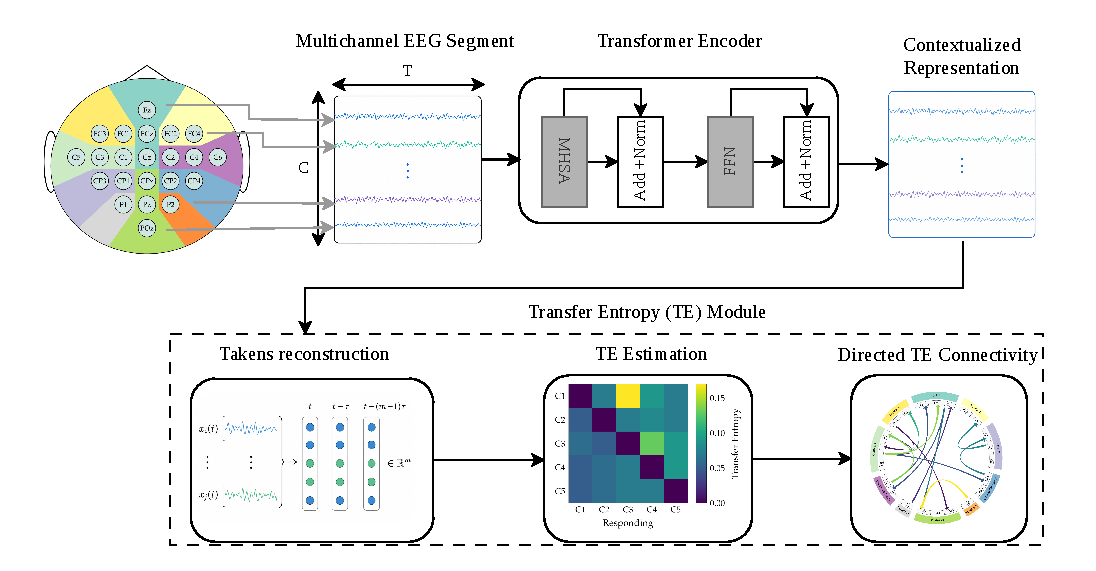
\includegraphics[width=\textwidth]{Figures/CTE-Net.pdf}
  \caption{Overview of the proposed framework for learning directed connectivity from multichannel \gls{eeg}. An input segment with $C$ channels and $T$ time samples is processed by a Transformer encoder comprising multi-head self-attention (MHSA), a feed-forward network (FFN), and residual connections with normalization (Add + Norm). The resulting contextualized representation enters the transfer entropy (TE) module, where Takens delay-coordinate reconstruction precedes the estimation of pairwise directed dependencies. These dependencies form a TE connectivity matrix, visualized as a directed connectivity graph.}
  \label{fig:tekte_pipeline}
\end{figure}

In this chapter, we extend the kernel-based TE paradigm to pediatric \gls{adhd} classification by proposing \gls{ctenet}, an end-to-end architecture that integrates Transformer-based contextualization with differentiable directed connectivity estimation. The model first processes each multichannel \gls{eeg} window using a Transformer encoder to obtain globally contextualized channel representations. These representations are then processed through channel-wise nonlinear temporal filters and Takens delay-coordinate embeddings. A differentiable kernel-based Transfer Entropy module estimates directed predictive information dependencies for all ordered electrode pairs, and the resulting connectivity representation is used for binary classification. In this manner, \gls{ctenet} combines global contextual modeling with nonlinear, time-delayed, and directed \gls{eeg} connectivity analysis.

Figure~\ref{fig:tekte_pipeline} illustrates the main processing stages of the proposed framework, from multichannel \gls{eeg} segments to directed-connectivity representations for \gls{adhd}-versus-control classification. A Transformer encoder produces contextualized representations, which are subsequently processed through Takens delay-coordinate reconstruction and transfer entropy estimation to characterize directed inter-channel dependencies.

\section{Materials and Methods}

{The original dataset comprised 61 participants with \gls{adhd} and 60 controls. To define a balanced cohort, one \gls{adhd} participant was randomly selected and excluded before window segmentation, fold construction, hyperparameter optimization, model training, and evaluation. The selection was not based on \gls{eeg} signal characteristics or quality, demographic or clinical information, model predictions, or classification performance. The resulting balanced cohort comprised 120 children, with 60 participants in the \gls{adhd} group and 60 in the control group, and was maintained across all models and experimental analyses.} The \gls{eeg} recordings were loaded in their original temporal form without applying additional artifact rejection, independent component analysis, frequency filtering, or spectral-band decomposition. This strategy was adopted to minimize preprocessing assumptions and allow the proposed network to learn temporal and connectivity-related patterns directly from the available multichannel recordings. As a post hoc signal-quality assessment, \gls{eeg} windows were screened for nonfinite values, flat channels, extreme amplitude, kurtosis, frontal low- and high-frequency activity, and 50-Hz line noise. Participant-balanced median/MAD thresholds were estimated from 30 windows per participant, with robust $z>5$ defining potentially contaminated windows. Without retraining, out-of-fold metrics were recalculated after excluding flagged windows and reaggregating participant probabilities; $z>4$ and $z>6$ were examined as sensitivity thresholds.

Each continuous recording was partitioned into 4-s windows, corresponding to 512 temporal samples at the original sampling frequency of 128~Hz. Consecutive windows were extracted with 50\% overlap; therefore, adjacent segments were separated by 256 samples, equivalent to a temporal shift of 2~s. The $n$-th \gls{eeg} segment was represented as

\begin{equation}
    \mathbf{X}^{(n)} \in \mathbb{R}^{C \times T},
\end{equation}

where $C=19$ is the number of \gls{eeg} channels and $T=512$ is the number of temporal samples per window. Each segment retained the diagnostic label and subject identifier associated with its original recording.

{The 50\% overlap increased temporal coverage and provided additional but partially redundant segments during model optimization; therefore, adjacent windows were not treated as independent statistical observations. Subject-wise partitioning kept all windows from each participant within a single training, validation, or test subset, preventing information leakage. Primary inference used one aggregated out-of-fold prediction per participant and participant-level bootstrap confidence intervals, while window-level metrics were interpreted as descriptive.}

{The number of windows per participant ranged from 30 to 167, with a median of 64 and an interquartile range of 51.75--77, yielding 8,213 windows in total. Participants with \gls{adhd} contributed 4,556 windows, with a median of 70.5 (IQR: 53.75--91.5), whereas controls contributed 3,657 windows, with a median of 59.5 (IQR: 51--68). Because training and window-level evaluation operated on individual windows, participants with longer recordings contributed more observations. Nevertheless, the primary participant-level evaluation assigned one aggregated out-of-fold prediction to each participant, giving all participants equal weight in the reported participant-level metrics.}

Subject identifiers were preserved throughout the experimental pipeline and subsequently used to construct the cross-validation partitions. Thus, all windows belonging to a given participant were assigned exclusively to a single training, validation, or test subset, preventing subject-level information leakage during model optimization and evaluation.
%------------------------------------------------------
\subsection{\gls{ctenet} Architecture}

\begin{table*}[htbp]
\centering
\caption{Compact \gls{ctenet} architecture for \gls{eeg}-based \gls{adhd} classification.}
\label{tab:model_architecture}

\small
\setlength{\tabcolsep}{5pt}
\renewcommand{\arraystretch}{1.17}

\begin{tabularx}{\textwidth}{@{}
    L{0.25\textwidth}
    L{0.13\textwidth}
    L{0.22\textwidth}
    Y
@{}}
\toprule
\textbf{Layer}
& \textbf{Variable}
& \textbf{Output dimension}
& \textbf{Configuration} \\
\midrule

\multicolumn{4}{@{}l}{\textbf{Block 1: Contextualization}} \\
\midrule

Input \gls{eeg}
& $\mat{X}$
& $C \times T$
& $C=19,\;T=512$ \\

Transpose
& $\mat{X}^{\top}$
& $T \times C$
& -- \\

Input projection
& $\mat{E}$
& $T \times d$
& {$d=128$} \\

Transformer encoder
& $\mat{H}$
& $T \times d$
& {$L=1,\;n_h=1,\;d_h=128,\;d_{ff}=128,\;p=0.5$} \\

Channel projection
& $\mat{X}_{f}^{\top}$
& $T \times C$
& $d\rightarrow C$ \\

Transpose
& $\mat{X}_{f}$
& $C \times T$
& -- \\

\midrule
\multicolumn{4}{@{}l}{\textbf{Block 2: Transfer Entropy}} \\
\midrule

Temporal filtering
& $\mat{\Phi}$
& $C \times T_{\phi}$
& {$K=83,\;T_{\phi}=107,\;s=1,\;\mathrm{pool}=4$} \\

Takens source state
& $\mat{Z}_{x^-}$
& $C \times T_z \times D_x$
& {$D_x=6,\;T_z=48$} \\

Takens target past
& $\mat{Z}_{y^-}$
& $C \times T_z \times D_y$
& {$D_y=1,\;T_z=48$} \\

Takens target present
& $\ve{z}_{y}$
& $C \times T_z \times 1$
& {$T_z=48$} \\

Kernel matrices
& $\mat{K}_{x^-},\,\mat{K}_{y^-},\,\mat{K}_{y}$
& {$19 \times 48 \times 48$}
& {$\tau=2,\;\mu=2,\;a=1,\;\ell=1,\;\alpha_{\mathrm{RQ}}=1$} \\

Transfer Entropy
& $\mat{TE}$
& $C \times C$
& $\alpha_{\mathrm{R}}=2$ \\

Flatten
& $\ve{h}_{TE}$
& $C(C-1)$
& -- \\

\midrule
\multicolumn{4}{@{}l}{\textbf{Block 3: Classification}} \\
\midrule

Dense
& $\ve{h}$
& $H$
& {$H=64$} \\

Dropout
& --
& {$64$}
& {$p=0.5$} \\

Output layer
& $\hat{y}$
& $O$
& $O=1$ \\

\bottomrule
\end{tabularx}
\end{table*}

% %----------------------------------------------------------------------------------

\subsubsection{Transformer-based contextualization}

Let a multichannel \gls{eeg} window be represented as $\mat{X}\in\mathbb{R}^{C\times T}$, where $C$ and $T$ denote the number of channels and temporal samples, respectively. Each temporal sample is treated as a sequence token containing the simultaneous activity of all \gls{eeg} channels. The normalized token sequence is projected onto a $d$-dimensional latent space as:

\begin{equation}
    \mat{E}
    =
    \operatorname{LN}_{C}\!\left(\mat{X}^{\top}\right)
    \mat{W}_{e}
    +
    \ve{b}_{e},
    \qquad
    \mat{E}\in\mathbb{R}^{T\times d}.
\end{equation}

A stack of $L$ standard Transformer encoder blocks \cite{vaswani2017attention}, comprising multi-head self-attention, feed-forward layers, residual connections, and layer normalization, produces

\begin{equation}
    \mat{H}
    =
    \operatorname{TrEnc}_{L}(\mat{E})
    \in\mathbb{R}^{T\times d}.
\end{equation}

The contextualized representation is projected back onto the original channel space:

\begin{equation}
    \mat{X}_{f}
    =
    \left[
        \operatorname{LN}(\mat{H})\mat{W}_{p}
        +
        \ve{b}_{p}
    \right]^{\top}
    \in\mathbb{R}^{C\times T}.
\end{equation}

Therefore, each row of $\mat{X}_{f}$ represents an \gls{eeg} channel contextualized using information from the complete temporal sequence and the remaining channels. The Transformer configuration is reported
in Table~\ref{tab:model_architecture}.

{No explicit positional encoding was incorporated into the Transformer encoder. Consequently, the self-attention mechanism does not, by itself, encode absolute temporal order or temporal distance based on token position. In \gls{ctenet}, self-attention is instead used as a content-based global contextualization mechanism, allowing each temporal sample to be represented in relation to the multichannel activity observed across the entire \gls{eeg} window. The resulting contextualized sequence remains indexed along the original time axis and is subsequently processed through channel-wise depthwise temporal convolution and Takens delay-coordinate reconstruction. These stages explicitly exploit temporal ordering and construct past and present states according to the reconstruction delay $\tau$ and the source--target interaction lag $\mu$. Thus, global content-based contextualization and the explicit modeling of ordered and delayed temporal dependencies are assigned to distinct components of the architecture.}

\subsubsection{Differentiable directed Transfer Entropy estimation}

The Transformer-contextualized signals are independently processed through channel-wise nonlinear temporal filters. The complete filtering operation is expressed as

\begin{equation}
    \mat{\Phi}
    =
    \operatorname{BN}
    \left[
        \operatorname{AvgPool}
        \left(
            \operatorname{ReLU}
            \left(
                \operatorname{DWConv1D}(\mat{X}_{f})
            \right)
        \right)
    \right]
    \in\mathbb{R}^{C\times T_{\phi}},
\end{equation}

where $\operatorname{DWConv1D}$ denotes a depthwise temporal convolution, so that each contextualized channel is filtered independently. The kernel size, stride, and pooling configuration are provided in
Table~\ref{tab:model_architecture}.

For each ordered source--target pair $(c,c')$, delay-coordinate embeddings are constructed from the filtered signals \cite{takens1981detecting}. At temporal anchor $t$, the source past, target past, and target present states are
defined as:

\begin{align}
    \ve{z}_{x_c^{-}}(t)
    &=
    \left[
        \phi_c(t-\mu-j\tau)
    \right]_{j=0}^{D_x-1}
    \in\mathbb{R}^{D_x},
    \\
    \ve{z}_{y_{c'}^{-}}(t)
    &=
    \left[
        \phi_{c'}(t-j\tau)
    \right]_{j=1}^{D_y}
    \in\mathbb{R}^{D_y},
    \\
    z_{y_{c'}}(t)
    &=
    \phi_{c'}(t).
\end{align}

Here, $D_x$ and $D_y$ are the source and target embedding dimensions, $\tau$ is the reconstruction delay, and $\mu$ represents the delayed source--target interaction.

Collecting the states over all valid temporal anchors yields $\mat{Z}_{x_c^{-}}$, $\mat{Z}_{y_{c'}^{-}}$, and $\mat{Z}_{y_{c'}}$. Before kernel evaluation, trainable bias-free
linear projections are applied:

\begin{equation}
    \widetilde{\mat{Z}}_{s}
    =
    \mat{Z}_{s}\mat{W}_{s},
    \qquad
    s\in
    \left\{
        x_c^{-},y_{c'}^{-},y_{c'}
    \right\}.
\end{equation}

For each projected state representation, a Gram matrix is constructed using the rational quadratic kernel \cite{rasmussen2006gaussian}. Specifically, for $s\in\{x_c^{-},y_{c'}^{-},y_{c'}\}$,

\begin{equation}
    \left[\mat{K}_{s}\right]_{ij}
    =
    \kappa_{\mathrm{RQ}}
    \left(
        \widetilde{\ve{z}}_{s,i},
        \widetilde{\ve{z}}_{s,j}
    \right)
    =
    a^{2}
    \left(
        1+
        \frac{
            \left\|
                \widetilde{\ve{z}}_{s,i}
                -
                \widetilde{\ve{z}}_{s,j}
            \right\|_{2}^{2}
        }{
            2\alpha_{\mathrm{RQ}}\ell^{2}
        }
    \right)^{-\alpha_{\mathrm{RQ}}},
\end{equation}

where $a$, $\ell$, and $\alpha_{\mathrm{RQ}}$ denote the kernel amplitude, length scale, and scale-mixture parameter, respectively.
The resulting matrices
$\mat{K}_{x_c^{-}}$, $\mat{K}_{y_{c'}^{-}}$, and $\mat{K}_{y_{c'}}$ encode pairwise similarities between the reconstructed states at the valid temporal anchors. The kernel configuration is reported in Table~\ref{tab:model_architecture}.
{For positive kernel parameters, the Rational Quadratic kernel produces positive-semidefinite Gram matrices. Moreover, the Hadamard products used to construct the joint kernel representations preserve positive semidefiniteness.}

{Numerical stability was ensured by enforcing strictly positive kernel parameters and using $\varepsilon=10^{-8}$ as a lower bound for the kernel length scale $\ell$ and shape parameter $\alpha_{\mathrm{RQ}}$, as well as a stabilizing constant during trace normalization and logarithmic entropy evaluation.}

For a positive semidefinite matrix $\mat{A}$, let the trace-normalization operator be defined as:

\begin{equation}
    \mathcal{N}(\mat{A})
    =
    \frac{\mat{A}}
    {\operatorname{tr}(\mat{A})}.
\end{equation}

The matrix-based R\'enyi entropy of order $\alpha_{\mathrm{R}}$ is then defined as:

\begin{equation}
    H_{\alpha_{\mathrm{R}}}(\mat{A})
    =
    \frac{1}{1-\alpha_{\mathrm{R}}}
    \log
    \left[
        \operatorname{tr}
        \left(
            \mathcal{N}(\mat{A})^{\alpha_{\mathrm{R}}}
        \right)
    \right].
\end{equation}
{This matrix-based entropy functional follows the positive definite kernel formulation introduced for information-theoretic learning and subsequently used for kernel-based Transfer Entropy estimation \cite{sanchezgiraldo2015entropy,delapava2019renyiTE}.}

For multiple variables represented by Gram matrices $\mat{K}_{1},\ldots,\mat{K}_{M}$, the corresponding joint entropy is computed from their Hadamard product:

\begin{equation}
    H_{\alpha_{\mathrm{R}}}
    \left(
        \mat{K}_{1},\ldots,\mat{K}_{M}
    \right)
    =
    H_{\alpha_{\mathrm{R}}}
    \left(
        \mat{K}_{1}
        \odot\cdots\odot
        \mat{K}_{M}
    \right),
\end{equation}

where $\odot$ denotes the Hadamard product. The trace normalization included in $H_{\alpha_{\mathrm{R}}}(\cdot)$ ensures that both marginal and joint kernel representations have unit trace before evaluating the entropy.

Accordingly, the directed Transfer Entropy from source channel $c$ to target channel $c'$ is computed as

\begin{align}
    TE_{c\rightarrow c'}
    ={}&
    H_{\alpha_{\mathrm{R}}}
    \left(
        \mat{K}_{y_{c'}^{-}},
        \mat{K}_{x_c^{-}}
    \right)
    -
    H_{\alpha_{\mathrm{R}}}
    \left(
        \mat{K}_{y_{c'}},
        \mat{K}_{y_{c'}^{-}},
        \mat{K}_{x_c^{-}}
    \right)
    \nonumber\\
    &+
    H_{\alpha_{\mathrm{R}}}
    \left(
        \mat{K}_{y_{c'}},
        \mat{K}_{y_{c'}^{-}}
    \right)
    -
    H_{\alpha_{\mathrm{R}}}
    \left(
        \mat{K}_{y_{c'}^{-}}
    \right).
\end{align}

Repeating this computation over all ordered channel pairs produces the directed connectivity matrix

\begin{equation}
    \mat{TE}
    =
    \left[
        TE_{c\rightarrow c'}
    \right]_{c,c'=1}^{C}
    \in\mathbb{R}^{C\times C}.
\end{equation}

Since the source and target states have different roles in the formulation, $\mat{TE}$ is generally asymmetric. Therefore, its coefficients represent directed predictive information dependencies
between Transformer-contextualized \gls{eeg} channels rather than undirected similarity relationships. {Although theoretical Transfer Entropy is non-negative, the present matrix-based formulation is a finite-sample estimator and does not explicitly enforce non-negativity. Consequently, negative estimates may occur and should not be interpreted as negative information transfer. Furthermore, because the Transformer, temporal filters, and linear projections preceding the TE module are optimized end-to-end using the supervised classification objective, the resulting coefficients quantify directed predictive dependencies within the learned representation space rather than conventional Transfer Entropy estimated directly from the raw \gls{eeg}. Accordingly, a labeled coefficient such as F8$\rightarrow$C4 denotes a directed dependency between channel-indexed coordinates of the learned contextualized representation and should not be interpreted as conventional Transfer Entropy between the original F8 and C4 electrode signals or as a source-level cortical interaction.}


\subsubsection{Connectivity-based classification}

The diagonal coefficients of $\mat{TE}$ represent self-connections and are excluded from the classification representation. The remaining directed coefficients are vectorized as

\begin{equation}
    \ve{h}_{\mathrm{TE}}
    =
    \operatorname{vec}
    \left(
        \left\{
            TE_{c\rightarrow c'}
            \mid
            c\neq c'
        \right\}
    \right)
    \in\mathbb{R}^{C(C-1)}.
\end{equation}

The resulting connectivity vector is processed by a fully connected classification head, and the estimated probability of \gls{adhd} is given by

\begin{equation}
    \hat{y}
    =
    \sigma
    \left[
        \ve{w}_{o}^{\top}
        \operatorname{Dropout}_{p_d}
        \left(
            \operatorname{ReLU}
            \left(
                \mat{W}_{h}\ve{h}_{\mathrm{TE}}
                +
                \ve{b}_{h}
            \right)
        \right)
        +
        b_o
    \right],
\end{equation}

where $\sigma(\cdot)$ denotes the sigmoid function and $p_d$ is the dropout probability. The complete architecture is optimized end-to-end using binary cross-entropy evaluated directly from the classification logits.

\subsection{Training Strategy and Evaluation Protocol}
\label{subsec:training_evaluation}

\gls{ctenet} was evaluated using five-fold stratified group cross-validation, with each participant treated as an independent group. At each iteration, 24 participants were held out for testing, while the remaining participants were divided into subject-independent training and validation subsets. Thus, no participant contributed windows to more than one subset, and each participant appeared once in the test set.

{The model was trained end-to-end at the window level using binary cross-entropy. A single hyperparameter configuration was selected through 20 Optuna trials \cite{akiba2019optuna}, using the mean validation accuracy across the five predefined subject-wise folds as the optimization objective. Within each fold, training, validation, and test participants were mutually exclusive, and only the corresponding validation subset guided early stopping and checkpoint selection. No test-set performance metric was included in hyperparameter optimization. The selected configuration, reported in Table~\ref{tab:model_architecture}, was then fixed for all five folds and all ten random training repetitions. Standardization and PCA were restricted to the post hoc representation analysis and did not influence model training, hyperparameter selection, or classification predictions.}

{Within the Transfer Entropy module, $D_x$, $D_y$, $\tau$, and $\mu$ were tuned through the 20-trial Optuna study over the ranges $D_x,D_y\in[1,10]$, $\tau\in[1,5]$, and $\mu\in[0,10]$. The selected values were $D_x=6$, $D_y=1$, $\tau=2$, and $\mu=2$. The Rényi order $\alpha_{\mathrm{R}}=2$ and the Rational Quadratic kernel parameters $a=\ell=\alpha_{\mathrm{RQ}}=1$ were fixed, whereas the linear projections preceding kernel evaluation were learned end-to-end.}

{A post hoc joint sensitivity analysis was conducted for $D_x$, $D_y$,
$\tau$, and $\mu$, as these parameters directly determine the temporal
organization of the reconstructed states and have shown relevant sensitivity
in related Takens-based kernel Transfer Entropy architectures
\cite{gomezrivera2025tektenet}. The originally selected configuration and ten feasible alternatives were evaluated across the five predefined subject-wise folds to characterize their combined sensitivity.}

The complete five-fold procedure was repeated using ten random seeds and identical subject partitions, resulting in 50 trained models. {The final \gls{ctenet} configuration contained 128,578 trainable parameters, corresponding to approximately 0.49~MiB of parameter storage in FP32. All experiments were conducted on the same workstation equipped with an NVIDIA Quadro RTX 5000 GPU, an eight-core CPU with 16 processing threads, and 16~GB of system RAM. The available execution records indicated approximate training times of 5--7 minutes per fold and 25--35 minutes for one complete five-fold repetition, while the complete 20-trial Optuna study required approximately 8.1 hours. For each \gls{eeg} window, the Transfer Entropy module evaluated all $C(C-1)=342$ ordered electrode pairs, excluding self-connections.} \gls{adhd} was considered the positive class, and window-level predictions were obtained using a probability threshold of 0.5. Performance was quantified as

\begin{equation}
\begin{aligned}
\mathrm{Accuracy}
&=\frac{\mathrm{TP}+\mathrm{TN}}
        {\mathrm{TP}+\mathrm{TN}+\mathrm{FP}+\mathrm{FN}},
&
\mathrm{Precision}
&=\frac{\mathrm{TP}}{\mathrm{TP}+\mathrm{FP}},
&
\mathrm{Sensitivity}
&=\frac{\mathrm{TP}}{\mathrm{TP}+\mathrm{FN}}.
\end{aligned}
\label{eq:classification_metrics}
\end{equation}

For each seed, metrics were averaged across the five test folds and reported as the mean and standard deviation across the ten seeds. \gls{ctenet} and the baselines were compared using paired two-sided Wilcoxon signed-rank tests with Holm correction {\cite{holm1979sequentially}}.

{These seed-based comparisons were retained as an exploratory assessment of the computational variability associated with repeated model training. The random seeds were not interpreted as independent clinical observations. Participant-level performance and uncertainty were therefore evaluated separately using the participants as the sampling units, as described below.}

{For the participant-level evaluation, the out-of-fold \gls{adhd} probabilities assigned to all windows belonging to participant $s$ under random training seed $r$ were averaged as}

\begin{equation}
{
\bar{p}_{s}^{(r)}
=
\frac{1}{N_s}
\sum_{i=1}^{N_s}
p_{s,i}^{(r)}
}
\label{eq:participant_probability}
\end{equation}

{where $N_s$ is the number of windows available for participant $s$ and $p_{s,i}^{(r)}$ is the \gls{adhd} probability assigned to window $i$. A participant was classified as \gls{adhd} when $\bar{p}_{s}^{(r)} \geq 0.5$ and as control otherwise. Accuracy, sensitivity, specificity, precision, and F1-score were calculated from the resulting participant-level decisions, whereas ROC-AUC was calculated directly from the continuous participant-level probabilities.}

{The participant-level metrics were calculated separately for each of the ten random training seeds using the 120 out-of-fold participants. Point estimates were subsequently obtained by averaging the corresponding metric across the ten seeds. The seeds were regarded as repeated model fits representing optimization variability and were not treated as independent clinical observations. Ninety-five percent confidence intervals were estimated using 5,000 stratified percentile bootstrap resamples at the participant level \cite{efron1979bootstrap}. Within each bootstrap replicate, control and \gls{adhd} participants were resampled separately with replacement, the same resampled participant indices were applied across all ten seeds, and the resulting seed-specific metrics were averaged.}

{All baseline architectures were trained and evaluated under the same experimental protocol as \gls{ctenet}, using identical training, validation, and test participant assignments, input windows, raw \gls{eeg} preprocessing, hyperparameter-tuning budget of 20 Optuna trials, validation-based early-stopping and checkpoint-selection criteria, and ten random training repetitions per fold. Although the hyperparameter search spaces were architecture-specific, the same optimization budget and validation objective were applied to every model.}

{Both ablation variants were evaluated using the same fixed subject-wise folds and ten random seeds as \gls{ctenet}. Seed-level differences were assessed using paired Wilcoxon signed-rank tests with Holm correction across six comparisons. For the participant-level analysis, one consensus decision per participant and model was obtained by averaging the out-of-fold probabilities across seeds and applying a threshold of 0.5. Exact McNemar tests \cite{mcnemar1947sampling} were then performed with Holm correction across the two ablation comparisons.}

{Sensitivity of predictive performance and learned connectivity to preprocessing and reference choice was assessed by retraining \gls{ctenet} using frequency-filtered and quality-screened \gls{eeg} or common average reference. Both analyses used the fixed configuration, five subject-wise folds, and ten seeds without additional hyperparameter optimization. Complete methods and results are provided in Supplementary Data~S4.}
\subsection{Representation Analysis}
\label{subsec:representation_analysis}

The original \gls{eeg}, Transformer output $\mat{X}_{f}$, temporal-filter output $\mat{\Phi}$, and Transfer Entropy representation were extracted exclusively from out-of-fold test windows. Each representation was vectorized, standardized within each seed--fold execution, and projected onto 30 principal components for the main analysis.

Let $\ve{z}_{s,i}^{(\ell,r)}$ denote the representation of window $i$ from participant $s$, at stage $\ell$ and repetition $r$. Within-subject dispersion and its change relative to the original \gls{eeg} were computed as:

\begin{equation}
\begin{aligned}
\boldsymbol{\mu}_{s}^{(\ell,r)}
&=\frac{1}{N_s}\sum_{i=1}^{N_s}\ve{z}_{s,i}^{(\ell,r)},
&
D_s^{(\ell,r)}
&=\frac{1}{N_s}\sum_{i=1}^{N_s}
\left\|
\ve{z}_{s,i}^{(\ell,r)}
-\boldsymbol{\mu}_{s}^{(\ell,r)}
\right\|_2,
\\
\widetilde{D}_s^{(\ell,r)}
&=\frac{D_s^{(\ell,r)}}{G^{(\ell,r)}},
&
\Delta_s^{(\ell)}
&=100\left(
\frac{\widetilde{D}_s^{(\ell)}}
     {\widetilde{D}_s^{(\mathrm{\gls{eeg}})}}
-1\right),
\end{aligned}
\label{eq:representation_dispersion}
\end{equation}

where $N_s$ is the number of windows and $G^{(\ell,r)}$ is the mean pairwise Euclidean distance among at most 1,200 test windows in the corresponding representation space. Participant-level dispersion was averaged across seeds before statistical analysis. Lower $\widetilde{D}_s^{(\ell,r)}$ values indicate more compact within-subject representations, whereas negative $\Delta_s^{(\ell)}$ values indicate a reduction relative to raw \gls{eeg}. These quantities describe representation-space dispersion rather than physiological \gls{eeg} variability.

Diagnostic organization was evaluated using the \gls{adhd}--control silhouette coefficient at the window level, the diagnostic silhouette of participant centroids \cite{rousseeuw1987silhouettes}, and the ratio $R=\overline{d}_{\mathrm{same}}/\overline{d}_{\mathrm{different}}$ between same-class and different-class centroid distances. Higher silhouette values and lower ratios indicate better diagnostic organization.

Finally, TE stability was evaluated by comparing each window-level connectivity vector with the mean of the remaining windows from the same participant. Spearman correlation measured the stability of the global connection ranking, while Jaccard similarity measured the overlap between the strongest 10\% of directed connections. Both measures were averaged across windows and seeds to obtain one value per participant.

Participant-level dispersion values were averaged across seeds and compared among stages using the Friedman test, followed by paired Wilcoxon signed-rank tests with Holm correction. Effect sizes were quantified using matched rank-biserial correlations, and 95\% confidence intervals were estimated from 5,000 participant-level bootstrap resamples. Robustness was assessed by repeating the analysis with 15, 30, and 60 PCA components and using pairwise cosine distance without PCA. Diagnostic-organization metrics were averaged across folds within each seed and analyzed using the same paired procedure.

{For each representation stage, the standardization mean and standard deviation and the PCA basis were computed independently from the pooled out-of-fold test windows of that stage and seed-fold, prior to projection onto the leading 30 components. Because this fitting is representation-specific,  we repeated the dispersion analysis using pairwise cosine distance on the standardized features without PCA, confirming that the reduction in within-subject dispersion is not an artifact of the per-representation standardization or PCA basis.}

%----------------------------------------------------------
\subsection{Results and Discussion}
\label{sec:results_and_discussion}
%----------------------------------------------------------
\gls{ctenet} was evaluated under the subject-independent protocol described in Section~\ref{subsec:training_evaluation}. The results examine four complementary aspects of the proposed architecture: classification performance and statistical comparison, model robustness and sensitivity, the organization and stability of the learned representation space, and subject-specific directed-connectivity patterns associated with correct and incorrect classification decisions.

\subsubsection{Classification Performance and Statistical Comparison}\label{subsec:classification_performance}

%----------------------------------------------------------
\begin{table}[htbp]
\centering
\caption{Window-level classification performance of \gls{ctenet} and the baseline models. Results are reported as the mean and sample standard deviation across ten random training seeds after averaging the five test folds within each seed.}
\label{tab:window_level_models}

\begin{threeparttable}
\scriptsize
\renewcommand{\arraystretch}{1.15}
\setlength{\tabcolsep}{3pt}

\begin{tabular*}{\textwidth}{@{\extracolsep{\fill}}l
    S[table-format=2.1]@{\,$\pm$\,}S[table-format=1.1]
    S[table-format=2.1]@{\,$\pm$\,}S[table-format=1.1]
    S[table-format=2.1]@{\,$\pm$\,}S[table-format=1.1]
    S[table-format=2.1]@{\,$\pm$\,}S[table-format=1.1]
    S[table-format=2.1]@{\,$\pm$\,}S[table-format=1.1]
    S[table-format=2.1]@{\,$\pm$\,}S[table-format=1.1]
    S[table-format=2.1]@{\,$\pm$\,}S[table-format=1.1]@{}}
\toprule

\multirow{2}{*}{\textbf{Model}}
& \multicolumn{4}{c}{\textbf{Overall}}
& \multicolumn{8}{c}{\textbf{Class-specific}}
& \multicolumn{2}{c}{\textbf{Ranking}} \\

\cmidrule(lr){2-5}\cmidrule(lr){6-13}\cmidrule(l){14-15}

& \multicolumn{2}{c}{\textbf{Accuracy}}
& \multicolumn{2}{c}{\textbf{BAcc}}
& \multicolumn{2}{c}{\textbf{Sens.}}
& \multicolumn{2}{c}{\textbf{Spec.}}
& \multicolumn{2}{c}{\textbf{Prec.}}
& \multicolumn{2}{c}{\textbf{F1}}
& \multicolumn{2}{c}{\textbf{ROC-AUC}} \\

\midrule

\rowproposed
\textbf{CTE-Net}
& 80.9 & 1.7 & 80.6 & 1.8 & 84.2 & 2.3 & 77.0 & 3.2 & 82.7 & 2.1 & 82.9 & 1.5 & 87.9 & 1.5 \\

\gls{eeg}Net
& 81.5 & 2.1 & 81.4 & 2.1 & 83.5 & 3.6 & 79.3 & 4.0 & 84.3 & 2.2 & 83.1 & 2.2 & 88.8 & 2.5 \\

ShallowConvNet
& \bfseries 83.5 & \bfseries 1.7 & \bfseries 83.7 & \bfseries 1.8 & 80.6 & 2.4 & \bfseries 86.9 & \bfseries 3.4 & \bfseries 88.1 & \bfseries 2.9 & \bfseries 83.2 & \bfseries 2.0 & \bfseries 90.4 & \bfseries 1.7 \\

T-GARNet
& 77.6 & 0.5 & 76.7 & 0.6 & 85.6 & 1.1 & 67.8 & 1.9 & 77.3 & 0.8 & 80.8 & 0.4 & 84.0 & 0.4 \\

IMC-BGT
& 66.3 & 1.2 & 65.3 & 1.4 & 74.7 & 2.7 & 55.8 & 4.5 & 68.2 & 1.6 & 70.8 & 1.0 & 71.2 & 1.0 \\

MultiStream
& 58.6 & 0.3 & 55.2 & 0.4 & \bfseries 86.1 & \bfseries 0.9 & 24.4 & 1.4 & 58.7 & 0.3 & 69.8 & 0.3 & 55.3 & 0.4 \\

\bottomrule
\end{tabular*}

\begin{tablenotes}[flushleft]
\footnotesize
\item \textit{Note:} All values are percentages. \gls{adhd} was treated as the
positive class, so sensitivity denotes the true-positive rate for \gls{adhd} and
specificity the true-negative rate for controls. BAcc denotes balanced
accuracy. Values were first averaged across the five test folds within each
seed and then summarized across the ten random training seeds. The seeds
represent repeated model fits and were not treated as independent clinical
observations. The shaded row indicates the proposed model, and bold values
indicate the highest point estimate for each metric.
\end{tablenotes}
\end{threeparttable}
\end{table}
%----------------------------------------------------------
{Classification performance was examined from two complementary statistical perspectives. First, the seed-level analysis characterized the variability associated with repeated model optimization under the same fixed subject-wise partitions. Mean and standard deviation across the ten random seeds were reported, and paired Wilcoxon signed-rank tests with Holm correction were used to assess whether the observed performance differences were consistent across repeated model fits. Because the subject partitions were reused, this analysis was interpreted as an assessment of optimization stability and not as inference based on independent clinical observations. Second, participant-level performance was evaluated using out-of-fold predictions, participant-level bootstrap confidence intervals, and exact paired McNemar tests, thereby treating the participant as the primary unit for evaluating generalization.}

{Table~\ref{tab:window_level_models} presents the complete window-level classification performance of \gls{ctenet} and the baseline models. In addition to accuracy, precision, and sensitivity, specificity, balanced accuracy, F1-score, and ROC-AUC are reported to provide a more complete assessment of class-specific behavior. These complementary metrics are particularly relevant for identifying models whose performance may be driven by a tendency to favor the \gls{adhd} class.}

{The window-level results reveal distinct classification profiles among the evaluated models. ShallowConvNet achieved the strongest overall point-estimate profile, leading in accuracy, balanced accuracy, specificity, precision, F1-score, and ROC-AUC, although it exhibited lower sensitivity than \gls{ctenet}. \gls{ctenet} and \gls{eeg}Net showed similarly competitive and comparatively balanced performance across the evaluated metrics, indicating that their classification results were not predominantly driven by either diagnostic class. In contrast, T-GARNet exhibited higher sensitivity but lower specificity and precision, suggesting a greater tendency to classify windows as \gls{adhd}. This behavior was even more pronounced for MultiStream, whose high sensitivity was accompanied by markedly lower specificity, balanced accuracy, precision, and ROC-AUC. IMC-BGT also showed a less balanced performance profile. Overall, these results demonstrate why sensitivity should be interpreted jointly with specificity, balanced accuracy, F1-score, and ROC-AUC when comparing the models.}

{The row-normalized window-level confusion matrices for all evaluated models are provided in Supplementary Data~S1. These matrices complement the reported class-specific metrics and facilitate inspection of each model's tendency to classify windows as \gls{adhd} or control.}

{To complement this descriptive performance analysis, the consistency of the differences between \gls{ctenet} and the baseline models across repeated training runs was examined using paired Wilcoxon signed-rank tests with Holm correction. These exploratory seed-level comparisons are reported in
Table~\ref{tab:ctenet_posthoc}.}

{Within the exploratory seed-level analysis, \gls{ctenet} and \gls{eeg}Net showed comparable accuracy, precision, and sensitivity across repeated model fits. ShallowConvNet achieved higher point estimates for accuracy and precision; however, only the precision difference remained significant after Holm correction. \gls{ctenet} showed consistently higher accuracy and precision than T-GARNet, IMC-BGT, and MultiStream. For sensitivity, \gls{ctenet} significantly outperformed only IMC-BGT, whereas no significant differences were found relative to \gls{eeg}Net, ShallowConvNet, T-GARNet, or MultiStream. Overall, these results indicate that \gls{ctenet} provides a stable balance among accuracy, precision, and sensitivity across repeated model fits.}
%----------------------------------------------------------
\begin{table}[htbp]
\centering
\caption{Exploratory seed-level comparisons between \gls{ctenet} and the
baseline models. Results are reported as the mean and standard deviation
across ten random training seeds. Paired Wilcoxon signed-rank tests were
used to evaluate the consistency of the differences across repeated
model fits, with Holm correction applied jointly across the 15
comparisons. Random seeds were treated as computational repetitions and
not as independent clinical observations.}
\label{tab:ctenet_posthoc}
\begin{threeparttable}
\scriptsize
\renewcommand{\arraystretch}{1.2}
\setlength{\tabcolsep}{3pt}
\begin{tabular*}{\textwidth}{@{\extracolsep{\fill}}l
    S[table-format=2.1]@{\,$\pm$\,}S[table-format=1.1] S[table-format=1.4] c
    S[table-format=2.1]@{\,$\pm$\,}S[table-format=1.1] S[table-format=1.4] c
    S[table-format=2.1]@{\,$\pm$\,}S[table-format=1.1] S[table-format=1.4] c@{}}
\toprule

\multirow{2}{*}{\textbf{Model}}
& \multicolumn{4}{c}{\textbf{Accuracy (\%)}}
& \multicolumn{4}{c}{\textbf{Precision (\%)}}
& \multicolumn{4}{c}{\textbf{Sensitivity (\%)}} \\

\cmidrule(lr){2-5}\cmidrule(lr){6-9}\cmidrule(l){10-13}

& \multicolumn{2}{c}{Mean\,$\pm$\,SD} & {$p_{\mathrm{Holm}}$} & vs.
& \multicolumn{2}{c}{Mean\,$\pm$\,SD} & {$p_{\mathrm{Holm}}$} & vs.
& \multicolumn{2}{c}{Mean\,$\pm$\,SD} & {$p_{\mathrm{Holm}}$} & vs. \\

\midrule

\rowproposed
\textbf{\gls{ctenet}}
& \textbf{80.9} & \textbf{1.7} & {--} & --
& \textbf{82.7} & \textbf{2.1} & {--} & --
& \textbf{84.2} & \textbf{2.3} & {--} & -- \\

\gls{eeg}Net
& 81.5 & 2.1 & 1.0000 & $\approx$
& 84.3 & 2.2 & 0.7734 & $\approx$
& 83.5 & 3.6 & 1.0000 & $\approx$ \\

ShallowConvNet
& \bfseries 83.5 & \bfseries 1.7 & 0.0684 & $\approx$
& \bfseries 88.1 & \bfseries 2.9 & 0.0293 & $<$
& 80.6 & 2.4 & 0.0820 & $\approx$ \\

T-GARNet
& 77.6 & 0.5 & 0.0293 & $>$
& 77.3 & 0.8 & 0.0293 & $>$
& 85.6 & 1.1 & 0.7734 & $\approx$ \\

IMC-BGT
& 66.3 & 1.2 & 0.0293 & $>$
& 68.2 & 1.6 & 0.0293 & $>$
& 74.7 & 2.7 & 0.0293 & $>$ \\

MultiStream
& 58.6 & 0.3 & 0.0293 & $>$
& 58.7 & 0.3 & 0.0293 & $>$
& \bfseries 86.1 & \bfseries 0.9 & 0.5273 & $\approx$ \\

\bottomrule
\end{tabular*}
\begin{tablenotes}[flushleft]
\footnotesize
\item \textit{Note:} All values are percentages. The shaded row shows
\gls{ctenet}'s own results, which serve as the reference for every comparison;
the ``vs.'' columns therefore contrast each baseline with \gls{ctenet}. The
symbols $>$ and $<$ indicate a Holm-adjusted difference across repeated
model fits in favor of \gls{ctenet} or the compared model, respectively;
$\approx$ indicates that no difference was detected. Bold values indicate
the highest point estimate for each metric. These comparisons characterize
optimization variability and should not be interpreted as participant-level
evidence of model superiority. Primary participant-level comparisons are
reported in Table~\ref{tab:participant_mcnemar}.
\end{tablenotes}
\end{threeparttable}
\end{table}
%----------------------------------------------------------

{Because \gls{adhd} diagnosis and the intended generalization unit correspond to the participant rather than to individual \gls{eeg} windows, performance was additionally evaluated after aggregating the out-of-fold window probabilities within each participant. Table~\ref{tab:subject_level_models} reports the resulting participant-level point estimates and 95\% confidence intervals for all evaluated models. The point estimates summarize performance across the ten repeated model fits, whereas the confidence intervals were obtained by resampling participants and therefore quantify uncertainty with respect to the study cohort.}

%----------------------------------------------------------
\begin{table}[htbp]
\centering
\caption{Participant-level classification performance of \gls{ctenet} and the baseline models. Point estimates correspond to the mean participant-level performance across ten random training seeds. The 95\% confidence intervals were estimated using 5,000 stratified bootstrap resamples with the participant as the resampling unit.}
\label{tab:subject_level_models}

\begin{threeparttable}
\scriptsize
\renewcommand{\arraystretch}{1.25}
\setlength{\tabcolsep}{3pt}

\begin{tabular*}{\textwidth}{@{\extracolsep{\fill}}lcccccc@{}}
\toprule

\multirow{2}{*}{\textbf{Model}}
& \multicolumn{2}{c}{\textbf{Overall}}
& \multicolumn{3}{c}{\textbf{Class-specific}}
& \multicolumn{1}{c}{\textbf{Ranking}} \\

\cmidrule(lr){2-3}\cmidrule(lr){4-6}\cmidrule(l){7-7}

& \textbf{Accuracy}
& \textbf{F1-score}
& \textbf{Sensitivity}
& \textbf{Specificity}
& \textbf{Precision}
& \textbf{ROC-AUC} \\

\midrule

\makecell{\textbf{CTE-Net}}
& \ci{83.4}{78.2--88.2}
& \ci{83.8}{78.7--88.4}
& \ci{86.0}{79.0--92.0}
& \ci{80.8}{73.2--87.7}
& \ci{81.8}{76.1--87.6}
& \ci{90.2}{85.1--94.6} \\

\makecell{\gls{eeg}Net}
& \ci{82.7}{77.7--87.3}
& \ci{83.4}{78.6--87.8}
& \ci{87.2}{80.5--92.7}
& \ci{78.2}{70.3--85.2}
& \ci{80.1}{74.5--85.8}
& \ci{89.2}{83.5--93.9} \\

\makecell{ShallowConvNet}
& \ci{\textbf{84.7}}{79.2--89.8}
& \ci{\textbf{84.4}}{78.3--89.7}
& \ci{82.5}{74.0--90.2}
& \ci{\textbf{87.0}}{80.0--92.8}
& \ci{\textbf{86.5}}{80.5--92.3}
& \ci{\textbf{91.6}}{86.6--95.7} \\

\makecell{T-GARNet}
& \ci{79.4}{72.5--85.8}
& \ci{81.4}{75.6--87.0}
& \ci{90.3}{82.5--96.8}
& \ci{68.5}{57.0--79.3}
& \ci{74.2}{67.6--81.4}
& \ci{85.8}{78.2--92.5} \\

\makecell{IMC-BGT}
& \ci{72.7}{66.3--78.8}
& \ci{75.8}{70.1--81.0}
& \ci{85.3}{77.0--92.3}
& \ci{60.0}{50.0--70.0}
& \ci{68.3}{62.7--74.4}
& \ci{78.6}{70.2--86.2} \\

\makecell{MultiStream}
& \ci{56.2}{51.2--61.4}
& \ci{68.2}{64.8--71.4}
& \ci{\textbf{93.7}}{88.3--98.0}
& \ci{18.8}{10.2--28.3}
& \ci{53.6}{50.6--56.8}
& \ci{60.3}{50.9--69.6} \\

\bottomrule
\end{tabular*}

\begin{tablenotes}[flushleft]
\footnotesize
\item \textit{Note:} All values are percentages; 95\% confidence intervals are
given in parentheses. For each participant and random seed, window-level \gls{adhd}
probabilities were averaged and a threshold of 0.5 was applied to obtain the
participant-level decision. Confidence intervals were calculated with the
participant as the resampling unit and quantify uncertainty around each model
separately; they should not be interpreted as tests of pairwise differences,
which are reported in Table~\ref{tab:participant_mcnemar}. The ten seeds
represent repeated model fits and were not treated as independent clinical
observations. Seed-level mean and standard deviation are reported separately
in Table~\ref{tab:ctenet_posthoc} as descriptive measures of optimization
variability. \gls{ctenet}, the proposed model, is listed first and set in bold;
bold values indicate the highest point estimate for each metric.
\end{tablenotes}
\end{threeparttable}
\end{table}
% %----------------------------------------------------------

{At the participant level, ShallowConvNet exhibited the strongest overall point-estimate profile, whereas \gls{ctenet} followed closely and achieved the second-highest accuracy, specificity, precision, F1-score, and ROC-AUC. \gls{eeg}Net also showed a competitive overall performance. In contrast, T-GARNet favored sensitivity at the expense of specificity and precision. This imbalance was more pronounced for IMC-BGT and particularly for MultiStream, indicating a greater tendency to classify participants as \gls{adhd}.}

{The participant-level estimates show that \gls{ctenet} maintained robust and comparatively balanced discrimination when each participant, rather than each \gls{eeg} window, was treated as the evaluation unit. Its joint sensitivity and specificity indicate that its performance was not driven exclusively by the classification of one diagnostic group. Nevertheless, the confidence intervals in Table~\ref{tab:subject_level_models} quantify uncertainty around each model separately and should not be interpreted as tests of pairwise differences. Formal paired comparisons were therefore conducted using the predictions obtained for the same participants.}

{To determine whether the descriptive performance differences translated into different classification outcomes for the same participants, one consensus decision was obtained for each participant and model by averaging the corresponding out-of-fold probabilities across the ten random seeds and applying the 0.5 threshold. \gls{ctenet} was then compared with each baseline using the exact McNemar test, with Holm correction across the five comparisons. Unlike the exploratory Wilcoxon analysis, this paired analysis used participants, rather than random seeds, as the units of comparison.}

% %----------------------------------------------------------
\begin{table}[H]
\centering
\caption{Exact participant-level McNemar comparisons between \gls{ctenet} and the baseline models. Consensus decisions were obtained by averaging each participant's out-of-fold probabilities across the ten random training seeds and applying a threshold of 0.5.}
\label{tab:participant_mcnemar}

\begin{threeparttable}
\small
\renewcommand{\arraystretch}{1.15}
\setlength{\tabcolsep}{5pt}

\begin{tabular*}{\textwidth}{@{\extracolsep{\fill}}l
    S[table-format=2.0]S[table-format=2.0]
    cc l@{}}
\toprule

\multirow{2}{*}{\textbf{Baseline}}
& \multicolumn{2}{c}{\textbf{Discordant participants}}
& \multicolumn{2}{c}{\textbf{Exact McNemar test}}
& \multirow{2}{*}{\textbf{vs.\ CTE-Net}} \\

\cmidrule(lr){2-3}\cmidrule(lr){4-5}

& {\boldmath$n_{10}$}
& {\boldmath$n_{01}$}
& \boldmath{$p_{\mathrm{exact}}$}
& \boldmath{$p_{\mathrm{Holm}}$}
& \\

\midrule

\gls{eeg}Net          &  8 & 7 & 1.0000 & 1.0000 & $\approx$ \\
ShallowConvNet  & 12 & 9 & 0.6636 & 1.0000 & $\approx$ \\
T-GARNet        & 12 & 3 & 0.0352 & 0.1055 & $\approx$ \\
IMC-BGT         & 21 & 7 & 0.0125 & 0.0502 & $\approx$ \\
MultiStream     & 47 & 9 & \boldmath{$2.57\times10^{-7}$} & \boldmath{$1.29\times10^{-6}$} & \boldmath{$>$} \\

\bottomrule
\end{tabular*}

\begin{tablenotes}[flushleft]
\footnotesize
\item \textit{Note:} $n_{10}$ denotes participants correctly classified by
\gls{ctenet} but incorrectly classified by the corresponding baseline, whereas
$n_{01}$ denotes participants incorrectly classified by \gls{ctenet} but correctly
classified by the baseline. Exact McNemar $p$-values were adjusted across the
five comparisons using the Holm procedure. The symbol $>$ indicates a
statistically significant difference favoring \gls{ctenet}, whereas $\approx$
indicates that no significant difference was found after Holm correction.
\end{tablenotes}
\end{threeparttable}
\end{table}

{As shown in Table~\ref{tab:participant_mcnemar}, the exact participant-level McNemar tests found no statistically significant differences between \gls{ctenet} and \gls{eeg}Net, ShallowConvNet, T-GARNet, or IMC-BGT after Holm correction. Although the unadjusted comparisons with T-GARNet and IMC-BGT reached the conventional significance threshold, these differences did not remain significant after correction for multiple comparisons. In contrast, \gls{ctenet} correctly classified significantly more participants than MultiStream after Holm correction.}

{The seed-level and participant-level analyses provide complementary evidence: the Wilcoxon results identify performance differences that were consistently reproduced across repeated model fits using the fixed participant partitions, whereas the McNemar results determine whether those differences translated into a significantly different number of correctly classified participants. Therefore, a difference may be stable across repeated model fits
without reaching statistical significance at the participant level after controlling for multiple comparisons.}

{Taken together, the results indicate that \gls{ctenet} does not uniformly outperform every strong classification baseline, but achieves competitive and comparatively balanced participant-level performance. No significant participant-level differences were detected between \gls{ctenet} and \gls{eeg}Net, ShallowConvNet, T-GARNet, or IMC-BGT, while a significant advantage over MultiStream was observed. Importantly, \gls{ctenet} complements this competitive predictive performance with an explicit representation of nonlinear, directed, and delayed interchannel dependencies, enabling the representation-level and connectivity analyses presented in the following sections.}

\subsubsection{Model Robustness and Sensitivity Analyses}
\label{subsec:model_robustness_sensitivity}

{To assess the robustness of the principal classification findings, a
post hoc signal-quality analysis identified 358 of 8,213 \gls{eeg} windows (4.36\%) as potentially contaminated under the primary robust threshold. Excluding these windows produced changes of no more than 0.51 percentage points in the window-level metrics and 0.17 percentage points in the participant-level metrics. Participant-level accuracy changed from 83.42\% to 83.50\%, while ROC-AUC changed from 90.24\% to 90.15\%. Moreover, the participant-level proportion of flagged windows was not significantly associated with the consensus \gls{adhd} probability across the complete cohort
($\rho=0.062$, $p=0.503$). These findings indicate that the principal results were stable after excluding windows with extreme signal-quality indicators. Detailed results are provided in Supplementary Data~S2.}

{Frequency filtering and quality screening, while retaining all participants, substantially reduced participant-level accuracy from 83.5\% to 73.9\% and ROC-AUC from 90.1\% to 81.9\%. In contrast, common average reference preserved classification performance but produced low agreement between the learned connectivity patterns ($\rho=0.070$; Jaccard $= 0.067$). These results indicate that \gls{ctenet} was sensitive to the combined cleaning procedure and that its detailed connectivity patterns depended on reference choice. Complete results are provided in Supplementary Data~S4.}

{Sensitivity to the architectural components was subsequently examined
through the component-wise ablation analysis reported in
Table~\ref{tab:ctenet_ablation}. The complete \gls{ctenet} architecture achieved
the highest point estimates across accuracy, sensitivity, and precision. Removing the Transformer produced the largest reductions across all three metrics. In the exploratory seed-level analysis, these differences remained significant after Holm correction for all three metrics ($p_{\mathrm{Holm}}=0.0117$). This result was also reflected at the participant level, where the exact McNemar comparison significantly favored the complete architecture. Replacing the Transfer Entropy module with temporal mean pooling also reduced the three point estimates; however, the seed-level difference was significant only for accuracy ($p_{\mathrm{Holm}}=0.0410$), and no significant participant-level difference was found. Therefore, the Transformer provides a clear predictive contribution, whereas the evidence for the predictive contribution of the Transfer Entropy module is more moderate. Nevertheless, the latter provides the explicit representation of nonlinear, delayed, and directed interchannel dependencies that distinguishes \gls{ctenet} from the pooling-based variant.}

%----------------------------------------------------------
\begin{table}[H]
\centering
\caption{Ablation study of \gls{ctenet}. Results are reported as the mean and sample standard deviation across ten random training seeds after averaging the five subject-wise test folds within each seed. The last column reports the primary participant-level exact McNemar comparisons against \gls{ctenet}.}
\label{tab:ctenet_ablation}

\begin{threeparttable}
\scriptsize
\renewcommand{\arraystretch}{1.15}
\setlength{\tabcolsep}{3pt}

\begin{tabular*}{\textwidth}{@{\extracolsep{\fill}}l
    cc l
    S[table-format=2.1]@{\,$\pm$\,}S[table-format=1.1]
    S[table-format=2.1]@{\,$\pm$\,}S[table-format=1.1]
    S[table-format=2.1]@{\,$\pm$\,}S[table-format=1.1]
    c@{}}
\toprule

\multirow{2}{*}{\textbf{Model variant}}
& \multicolumn{3}{c}{\textbf{Architecture}}
& \multicolumn{6}{c}{\textbf{Window-level performance (\%)}}
& \multicolumn{1}{c}{\textbf{Participant level}} \\

\cmidrule(lr){2-4}\cmidrule(lr){5-10}\cmidrule(l){11-11}

& \textbf{Trans.}
& \textbf{TE}
& \textbf{Representation}
& \multicolumn{2}{c}{\textbf{Accuracy}}
& \multicolumn{2}{c}{\textbf{Sensitivity}}
& \multicolumn{2}{c}{\textbf{Precision}}
& \boldmath{$p_{\mathrm{Holm}}$} \\

\midrule

Without Transformer
& $\times$ & $\checkmark$ & Rational quadratic
& 73.4 & 2.2 & 78.0 & 2.8 & 75.7 & 2.5
& $\mathbf{0.0338}$ \\

Without TE module
& $\checkmark$ & $\times$ & Temporal mean pooling
& 78.7 & 0.8 & 82.3 & 2.8 & 80.8 & 1.6
& $0.2891$ \\

\rowproposed
\textbf{CTE-Net (proposed)}
& $\checkmark$ & $\checkmark$ & Rational quadratic
& \bfseries 80.9 & \bfseries 1.7 & \bfseries 84.2 & \bfseries 2.3 & \bfseries 82.7 & \bfseries 2.1
& -- \\

\bottomrule
\end{tabular*}

\begin{tablenotes}[flushleft]
\footnotesize
\item \textit{Note:} All variants were evaluated using the same fixed
subject-wise folds and ten random training seeds. The seeds represent repeated
model fits and were not treated as independent clinical observations.
Participant-level comparisons were performed using one consensus decision per
participant and model. Exact McNemar $p$-values were adjusted across the two
ablation comparisons using the Holm procedure. Bold $p$-values indicate
statistically significant differences favoring \gls{ctenet} after correction, and
the shaded row indicates the complete architecture.
\end{tablenotes}
\end{threeparttable}
\end{table}
%----------------------------------------------------------

{The contribution of the Transfer Entropy module should not be interpreted solely in terms of predictive performance. Replacing it with temporal mean pooling removes the explicit representation of nonlinear, time-delayed, and directional interchannel relationships. Although the participant-level predictive difference between the complete architecture and the pooling-based variant was not statistically significant, \gls{ctenet} preserved an explicit and inspectable directed-connectivity space. This contribution is further supported by the subsequent representation analyses, in which the TE stage produced a more compact within-subject organization, remained consistent across alternative PCA dimensionalities and distance definitions, and enabled the inspection of subject-specific directed-connectivity patterns.}

{Finally, a post hoc structural sensitivity analysis showed that mean
validation accuracy across the 11 configurations ranged from 81.63\% to 89.78\%, with a median of 86.20\%, indicating sensitivity to the joint selection of $D_x$, $D_y$, $\tau$, and $\mu$. Although several post hoc alternatives exceeded the originally selected configuration in validation, they were not evaluated under the repeated test protocol. Moreover, because the parameters were varied jointly, these results neither identify individual effects nor establish superior generalization. Complete results are provided in Supplementary
Data~S3.}

\subsubsection{Evolution and Diagnostic Organization of the Learned Feature Space} \label{subsec:feature_space_evolution}

Figure~\ref{fig:tsne_architecture_stages} qualitatively illustrates the progressive reorganization of the \gls{eeg} representation across \gls{ctenet}. The raw \gls{eeg} windows exhibit substantial overlap between \gls{adhd} and control participants. Transformer contextualization produces a more structured distribution, although local overlap and participant-dependent subclusters remain. This organization becomes progressively clearer after nonlinear temporal filtering and is most pronounced in the directed Transfer Entropy representation, which shows the most favorable visual arrangement of the two diagnostic groups.

Because a separate t-SNE projection was fitted to each representation, the axes, scales, and absolute distances are not directly comparable across panels. Therefore, Figure~\ref{fig:tsne_architecture_stages} is interpreted exclusively as qualitative evidence, whereas diagnostic organization was quantified in the standardized PCA space using the metrics reported in Table~\ref{tab:diagnostic_organization}.

\begin{figure}[H]
    \centering
    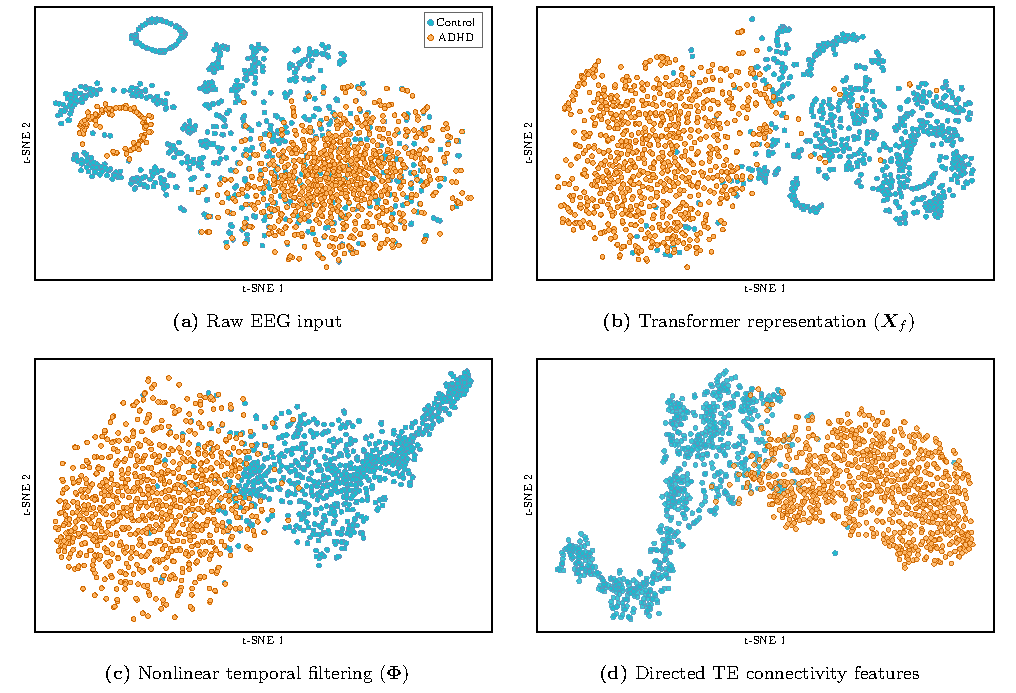
\includegraphics[width=\textwidth]
    {Figures/T-Sne}

    \caption{Evolution of the \gls{eeg} feature space across the main stages of \gls{ctenet}. The t-SNE projections correspond to (a) the raw \gls{eeg} input, (b) Transformer-contextualized channel representations, (c) nonlinear temporal filtering, and (d) directed transfer entropy connectivity features. Blue and orange markers denote Control and \gls{adhd}, respectively.}
    \label{fig:tsne_architecture_stages}
\end{figure}

The quantitative results in Table~\ref{tab:diagnostic_organization} corroborate the progressive organization observed in the t-SNE projections. The raw \gls{eeg} space showed weak diagnostic structure, with participant centroids from the same class being nearly as distant as those from different classes. Transformer contextualization improved this organization primarily at the participant level, despite the remaining overlap among individual windows. Nonlinear temporal filtering further enhanced both window- and centroid-level organization.

The Transfer Entropy representation achieved the most favorable result for all three metrics. Although some \gls{adhd}--control overlap remained, the simultaneous increase in both silhouette coefficients and reduction in the centroid-distance ratio indicate a more coherent diagnostic organization. Differences among stages were significant for all metrics (Friedman tests, $p\leq 3\times10^{-6}$), and the comparisons between the raw \gls{eeg} and Transfer Entropy spaces remained significant after Holm correction ($p_{\mathrm{Holm}}=0.0117$). Therefore, the qualitative t-SNE pattern is supported by quantitative evidence computed in the
standardized PCA space and does not depend exclusively on the two-dimensional visualization. These findings also indicate that the subsequent reduction in within-subject dispersion was not achieved at the expense of \gls{adhd}--control organization.

\begin{table}[htbp]
\centering
\caption{Diagnostic organization across the representation stages of \gls{ctenet}. Values correspond to averages across the ten training repetitions after averaging the five test folds within each repetition.}
\label{tab:diagnostic_organization}

\begin{threeparttable}
\small
\renewcommand{\arraystretch}{1.20}
\setlength{\tabcolsep}{5pt}

\begin{tabular*}{\textwidth}{@{\extracolsep{\fill}}l
    S[table-format=1.4]S[table-format=1.4]S[table-format=1.4]@{}}
\toprule

\textbf{Representation}
& \multicolumn{2}{c}{\textbf{Class silhouette} $\uparrow$}
& {\textbf{Same/different}} \\

\cmidrule(lr){2-3}

\textbf{stage}
& {\textbf{Window level}}
& {\textbf{Centroid level}}
& {\textbf{class ratio}\,$\downarrow$} \\

\midrule

Raw \gls{eeg}                  & 0.0558 & 0.0210 & 0.9887 \\
Transformer ($X_f$)      & 0.0712 & 0.2640 & 0.7056 \\
Temporal filter ($\Phi$) & 0.1326 & 0.3316 & 0.6326 \\
Transfer Entropy         & \bfseries 0.2148 & \bfseries 0.3557 & \bfseries 0.6031 \\

\bottomrule
\end{tabular*}

\begin{tablenotes}[flushleft]
\footnotesize
\item \textit{Note:} Arrows indicate the direction of more favorable
diagnostic organization: higher silhouette coefficients ($\uparrow$) and lower
same-to-different class centroid-distance ratios ($\downarrow$). All
quantities were computed in the standardized PCA space described in
Section~\ref{subsec:representation_analysis}. Bold values indicate the most
favorable value for each measure, obtained in every case at the directed
Transfer Entropy stage.
\end{tablenotes}
\end{threeparttable}
\end{table}
%----------------------------------------------------------
\subsubsection{Reduction of Within-Subject Variability across \gls{ctenet} Representations}


Figure~\ref{fig:within_subject_dispersion} shows the evolution of normalized within-subject dispersion across the four representation stages. The raw \gls{eeg} representation exhibited substantial between-participant heterogeneity, including several subjects with markedly elevated dispersion. Transformer contextualization produced a narrower distribution across participants, but did not reduce the median dispersion relative to raw \gls{eeg}. In contrast, nonlinear temporal filtering initiated a reduction, which became most pronounced after the directed Transfer Entropy transformation.

\begin{figure}[htbp]
    \centering
    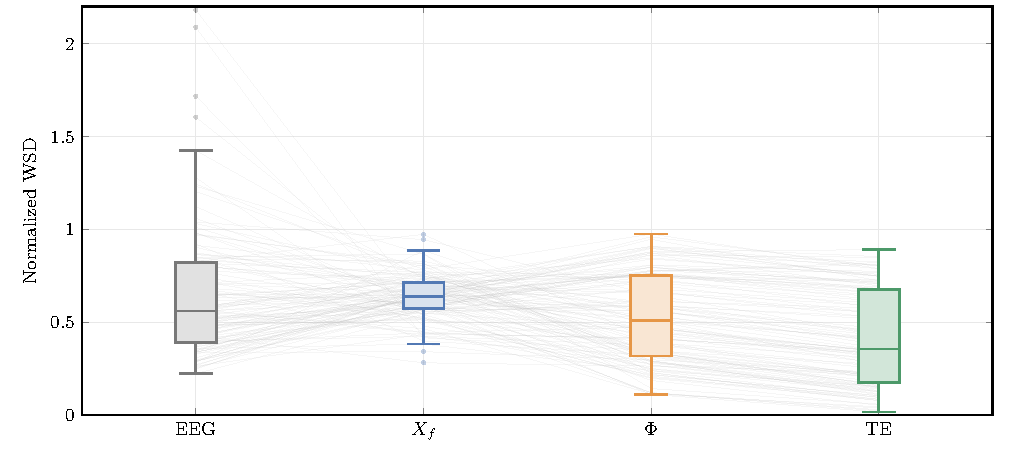
\includegraphics[width=\textwidth]{Figures/Dispersion.pdf}
    \caption{Within-subject dispersion across the four representation stages of \gls{ctenet}. Boxplots summarize the normalized subject-level
    dispersion after averaging across ten random seeds, while the faint trajectories connect the four representations of each participant.
    Lower values indicate a more compact organization of \gls{eeg} windows within the same participant. The directed Transfer Entropy
    representation exhibited the lowest overall within-subject dispersion.}
    \label{fig:within_subject_dispersion}
\end{figure}
% %----------------------------------------------------------

The Transfer Entropy representation exhibited the lowest median and mean within-subject dispersion among all stages. Relative to raw \gls{eeg}, the median reduction was 38.35\%, with lower dispersion observed in 76 of the 120 participants. This reduction was statistically supported by the Holm-corrected Wilcoxon comparison ($p_{\mathrm{Holm}}=1.09\times10^{-4}$), while the overall differences among representation stages were significant according to the Friedman test ($\chi^2(3)=69.11$, $p=6.62\times10^{-15}$). Although individual trajectories were heterogeneous and the reduction was not observed for every participant, the overall pattern indicates that directed-connectivity estimation produces a more compact organization of windows belonging to the same child.

{A reduction in within-subject dispersion would not be meaningful if it resulted from a general collapse of the representation space. Two complementary findings argue against a simple global collapse. First, the dispersion measure is normalized by the mean pairwise distance across the complete test set within each representation; therefore, a uniform contraction would reduce both the within-subject and reference distances proportionally and would not, by itself, explain the observed change. Second, the Transfer Entropy stage simultaneously exhibited the most favorable diagnostic organization, including the highest window- and centroid-level silhouette coefficients and the lowest same-class to different-class centroid-distance ratio (Table~\ref{tab:diagnostic_organization}). The cosine-distance analysis without PCA separately confirmed that the reduction in within-subject dispersion was not an artifact of the PCA basis or Euclidean geometry. Together, these findings argue against a simple global feature collapse, although they do not exclude every possible form of representation degeneration.}

\subsubsection{Robustness to the comparison space}

To determine whether the observed reduction in within-subject dispersion depended on the dimensionality or geometry selected for the analysis, the representations were evaluated using PCA projections with 15, 30, and 60 components, as well as pairwise cosine distances computed directly from the standardized features without PCA. As shown in Fig.~\ref{fig:robustness_representation_space}, the intermediate Transformer representation exhibited a moderate increase in dispersion under the PCA-based configurations, whereas the nonlinear temporal filtering stage produced a consistent reduction relative to the raw \gls{eeg} representation. Most importantly, the Transfer Entropy representation yielded the largest reduction under all evaluated comparison spaces, with median changes of approximately 37--45\%. The similar results obtained with 15, 30, and 60 principal components indicate that the effect is not determined by the specific PCA dimensionality selected for the main analysis.

% %----------------------------------------------------------
\begin{figure}[htbp]
    \centering
    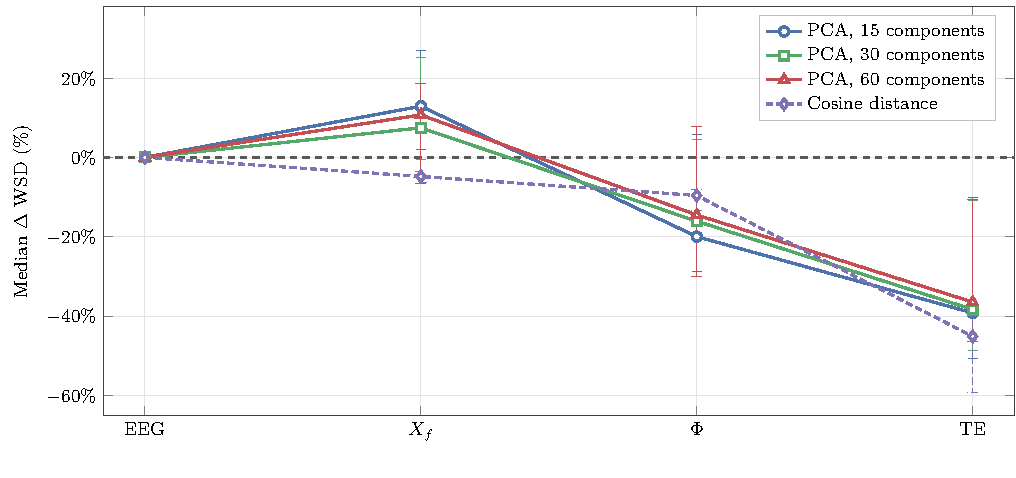
\includegraphics[width=\textwidth]{Figures/Robustness.pdf}
    \caption{Robustness of within-subject dispersion reduction across alternative comparison spaces. The median percentage change in normalized within-subject dispersion is shown relative to the raw \gls{eeg} representation for PCA projections with 15, 30, and 60 components, and for pairwise cosine distances computed without PCA. Negative values indicate a reduction in within-subject dispersion, while the vertical bars represent 95\% bootstrap confidence intervals.}
    \label{fig:robustness_representation_space}
\end{figure}
% %----------------------------------------------------------
The preservation of the effect when using cosine distances without PCA further indicates that the reduction is not an artifact introduced by the linear projection or by the Euclidean centroid-based geometry. Although the magnitude of the reduction varied across comparison spaces, its direction remained consistent at the Transfer Entropy stage. This result supports the interpretation that the directed-connectivity transformation produces a more compact organization of the windows belonging to the same participant. Therefore, the main finding of reduced within-subject dispersion is robust to alternative dimensionality-reduction settings and distance definitions, complementing the subject-level Friedman and Wilcoxon analyses reported previously.

\subsubsection{Stability of Directed Transfer Entropy Representations}

{Across the out-of-fold test representations, the off-diagonal Transfer Entropy coefficients ranged from $-0.0801$ to $0.5156$. Negative estimates accounted for $10.06\%$ of the coefficients, and no non-finite values were observed. The negative values were retained rather than clipped because non-negativity is not explicitly imposed by the finite-sample matrix-based estimator and should not be interpreted as negative information transfer.}

{Across the 120 participants, the mean Spearman correlation between each window-level Transfer Entropy vector and the mean of the participant's remaining windows was 0.743 (95\% CI: 0.733--0.753). The mean Jaccard similarity for the strongest 10\% of directed connections was 0.492 (95\% CI: 0.474--0.509). These results indicate that the global ranking of directed connections remained comparatively stable across windows, whereas the exact composition of the strongest connections showed greater variability.}

\subsubsection{Subject-level analysis of directed connectivity patterns}

To qualitatively illustrate subject-level connectivity patterns associated with correct and incorrect model decisions, four participants were selected from the held-out test partition using their participant-level classification probabilities. These probabilities were obtained by averaging the predicted \gls{adhd} probabilities across all windows of each participant. The correctly classified Control and \gls{adhd} cases corresponded to the lowest and highest mean \gls{adhd} probabilities within their respective classes, whereas the misclassified Control and \gls{adhd} cases corresponded to the opposite extremes. The connectivity maps themselves were not used in the selection procedure. For each selected participant, the displayed Transfer Entropy matrix was obtained by averaging the connectivity matrices across all available \gls{eeg} windows.
% %----------------------------------------------------------------------------------
\begin{figure}[H]
    \centering

    \begin{minipage}[c]{0.44\textwidth}
        \centering
        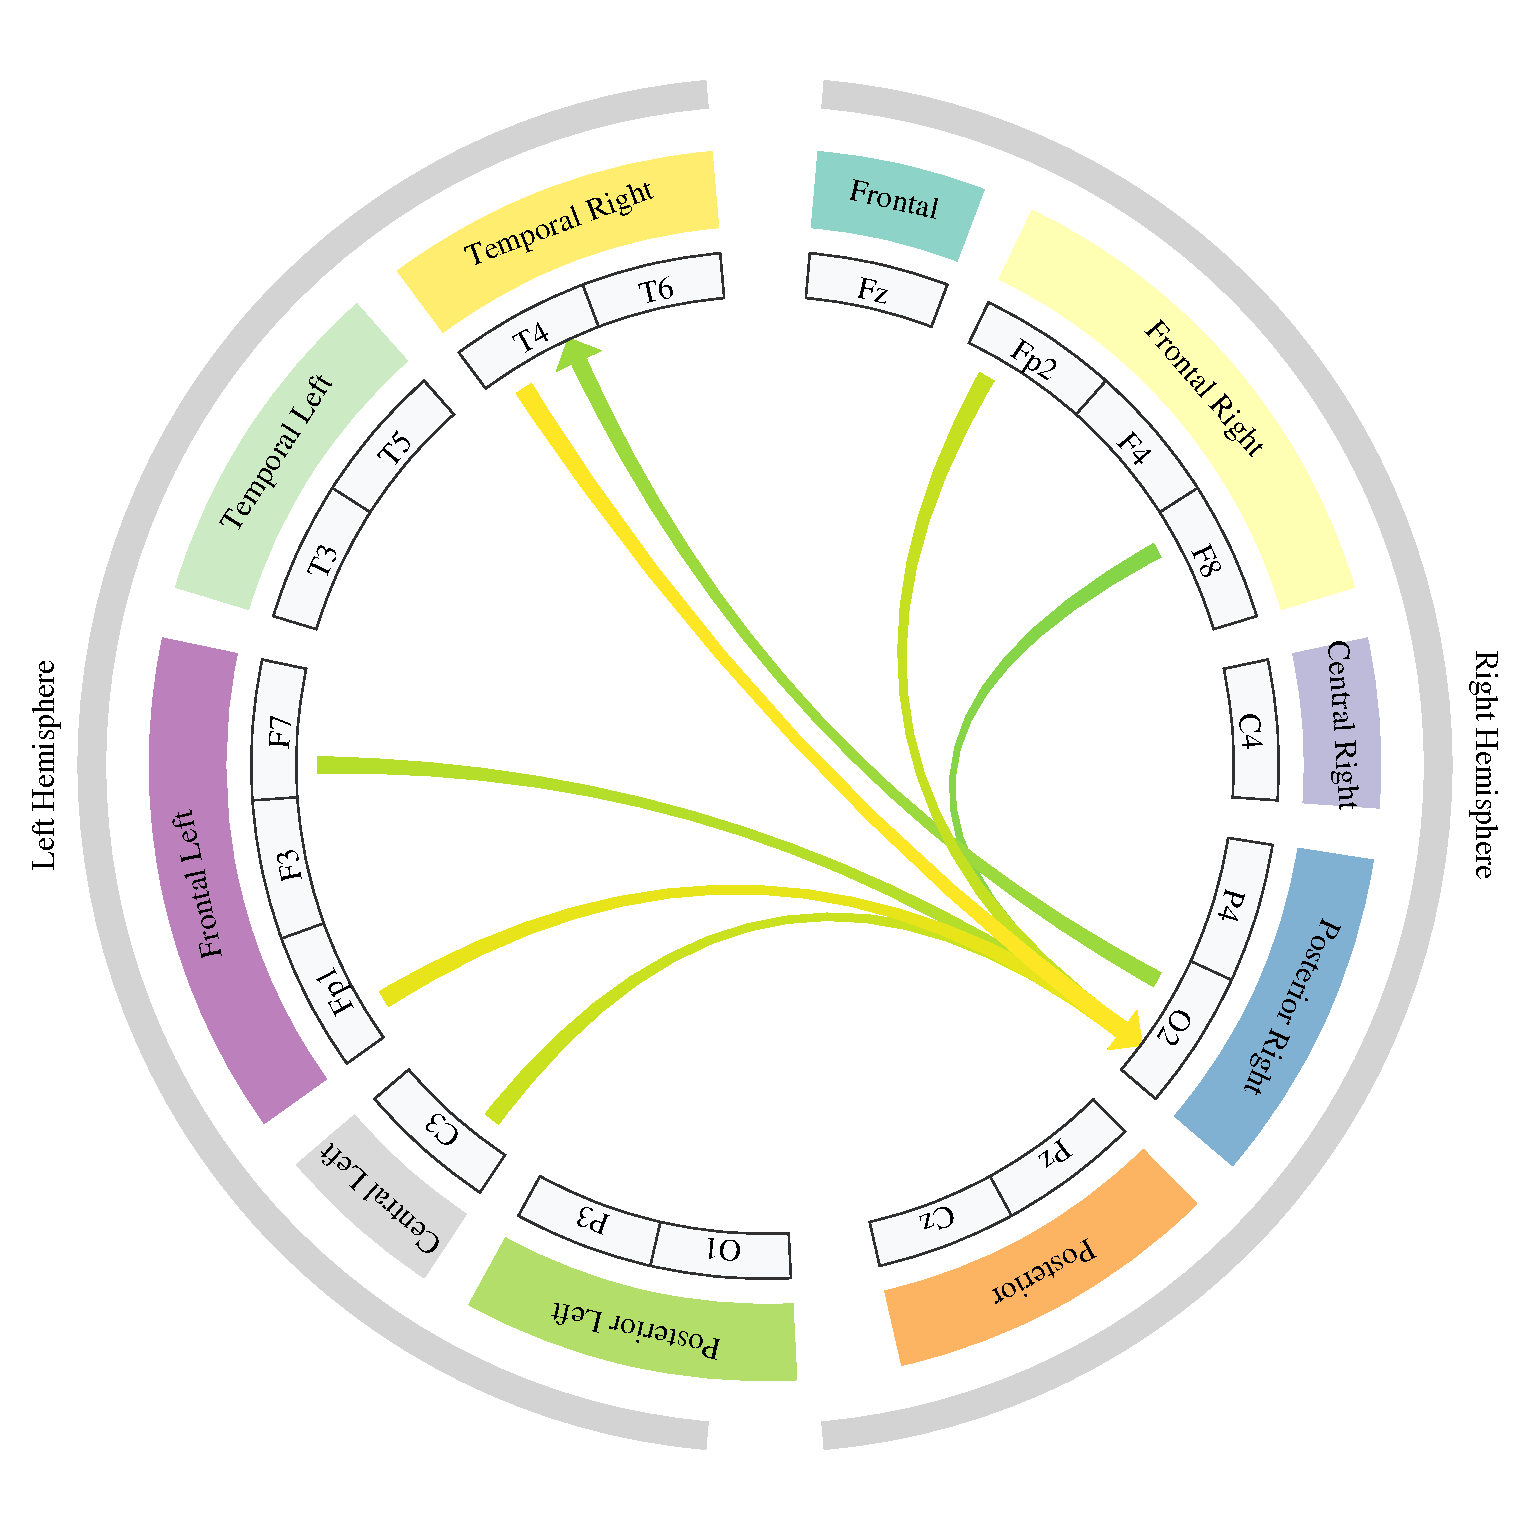
\includegraphics[
            width=\linewidth
        ]{Figures/best_control_v306_normalized.pdf}

        \vspace{1mm}

        {\small
        (a) Correctly classified Control (\texttt{Sv306}).}
    \end{minipage}
    \hfill
    \begin{minipage}[c]{0.44\textwidth}
        \centering
        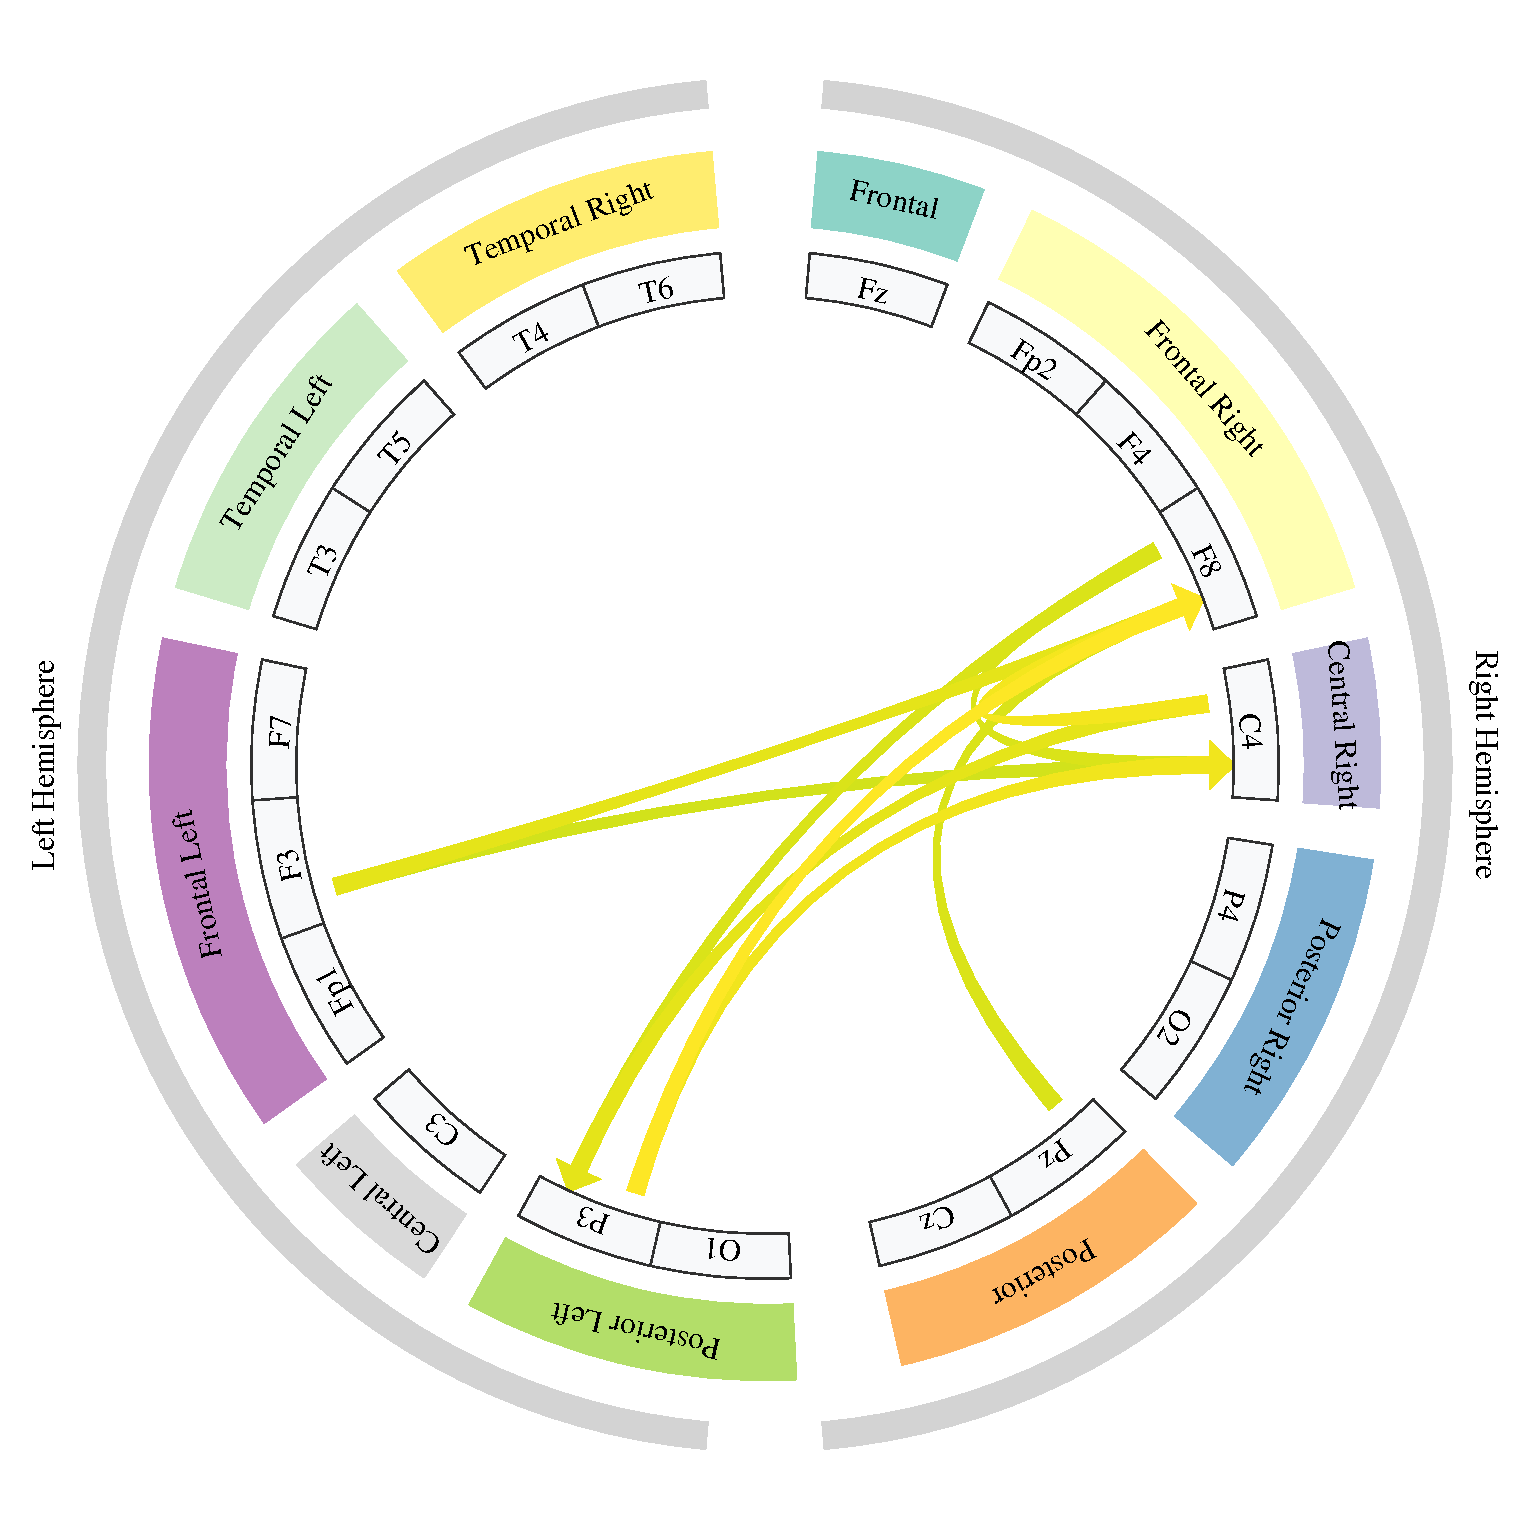
\includegraphics[
            width=\linewidth
        ]{Figures/best_tdah_v284_normalized.pdf}

        \vspace{1mm}

        {\small
        (b) Correctly classified \gls{adhd} (\texttt{Sv284}).}
    \end{minipage}
    \hfill
    \begin{minipage}[c]{0.055\textwidth}
        \centering

        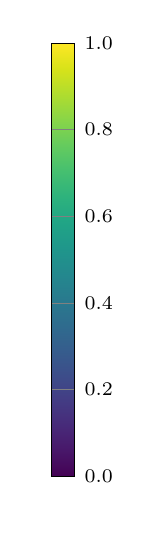
\begin{tikzpicture}
            \begin{axis}[
                hide axis,
                scale only axis,
                width=0pt,
                height=6.5cm,
                colormap/viridis,
                point meta min=0,
                point meta max=1,
                colorbar,
                colorbar style={
                    height=5.5cm,
                    width=0.30cm,
                    ytick={0,0.2,0.4,0.6,0.8,1},
                    yticklabels={0.0,0.2,0.4,0.6,0.8,1.0},
                    yticklabel style={
                        font=\scriptsize
                    }
                }
            ]

            \addplot[
                draw=none,
                point meta=explicit
            ]
            coordinates {
                (0,0) [0]
                (1,1) [1]
            };

            \end{axis}
        \end{tikzpicture}
    \end{minipage}

    \caption{
        Directed Transfer Entropy connectivity patterns for
        representative correctly classified subjects.
        Only the top 5\% of the strongest directed connections are shown.
        Arrow direction indicates the estimated direction of information
        transfer, while color represents the normalized TE magnitude
        using a shared range.
    }

    \label{fig:correct_subjects_te}
\end{figure}

% %----------------------------------------------------------------------------------

\begin{figure}[H]
    \centering

    \begin{minipage}[c]{0.445\textwidth}
        \centering
        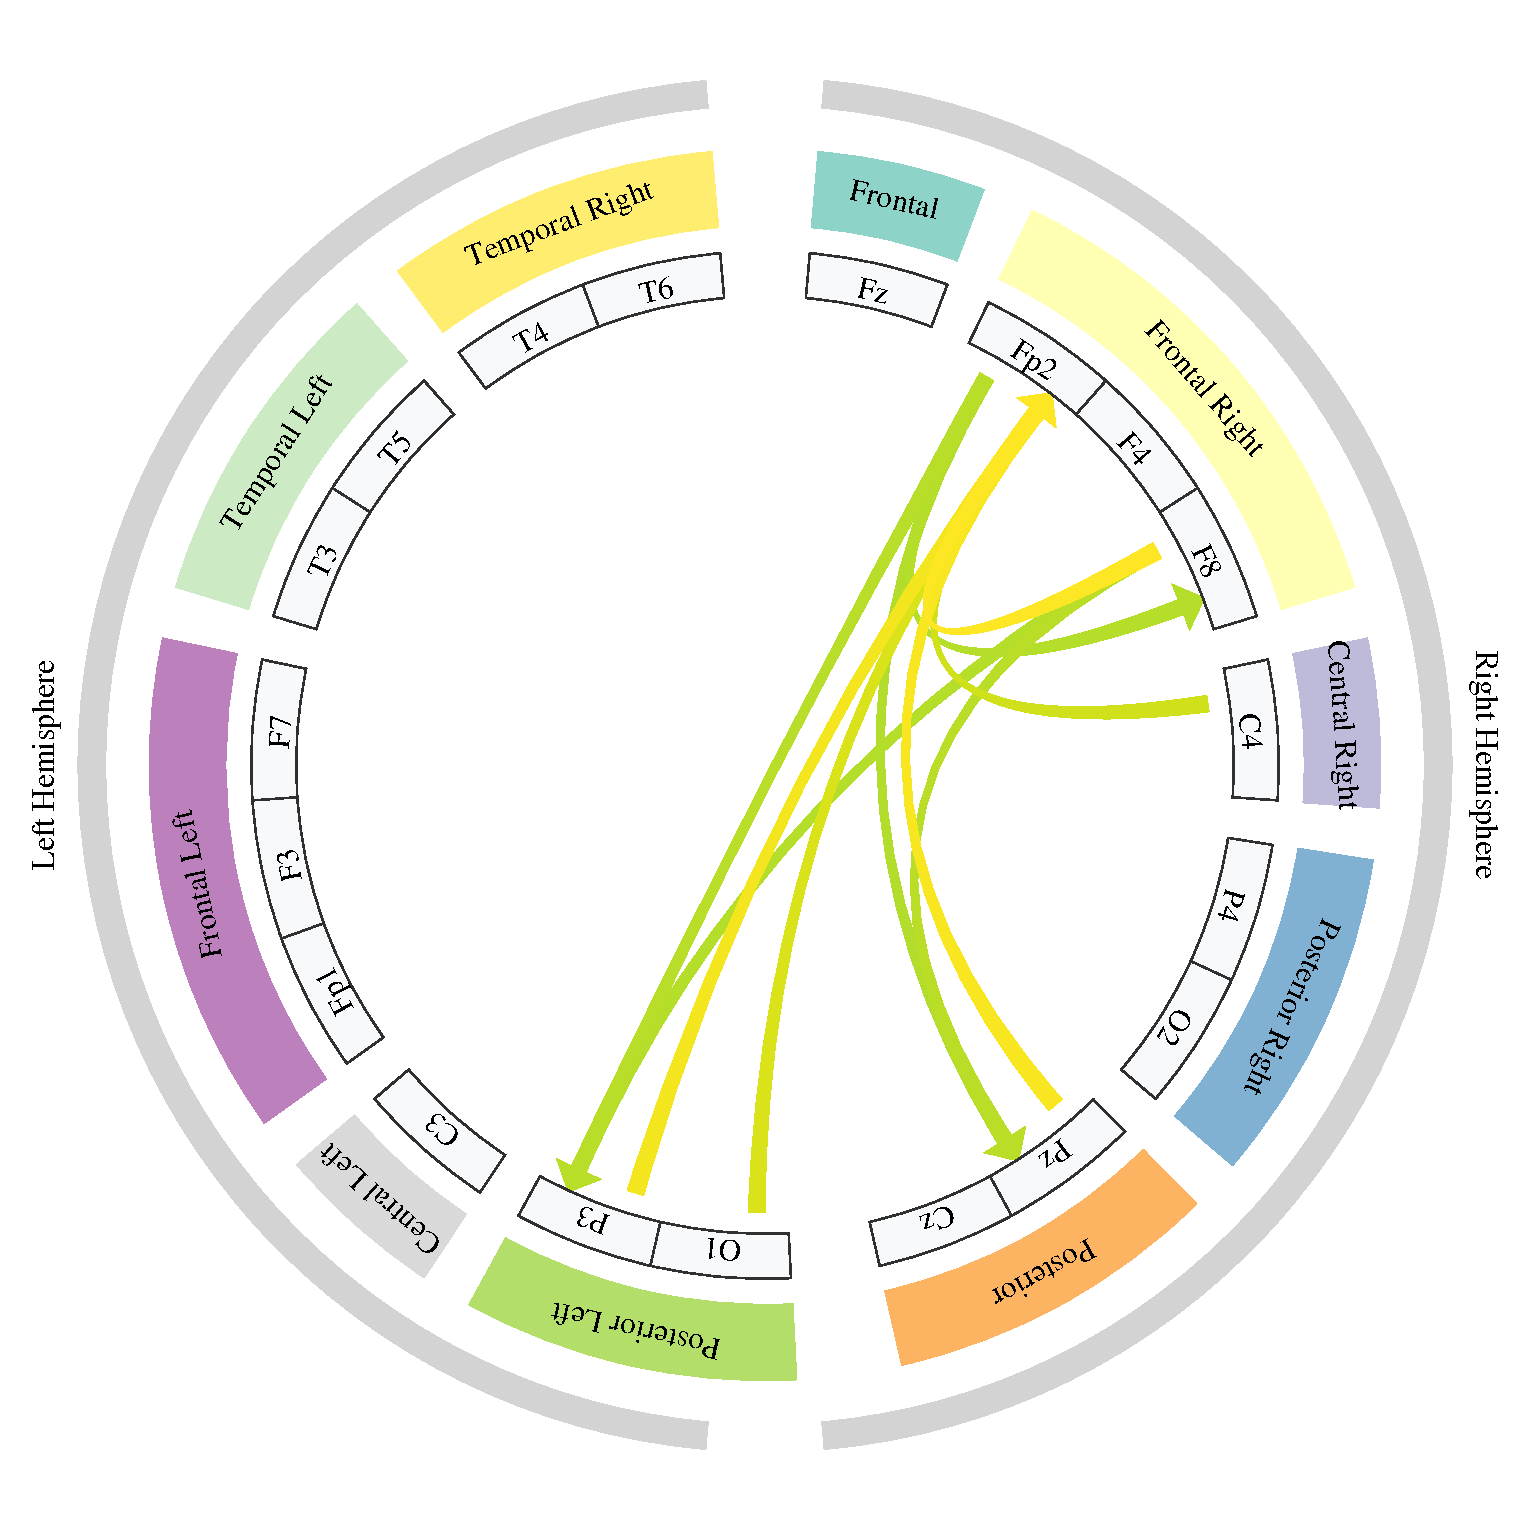
\includegraphics[
            width=\linewidth
        ]{Figures/misclassified_control_v297_normalized.pdf}

        \vspace{1mm}

        {\small
        (a) Misclassified Control (\texttt{Sv297}).}
    \end{minipage}
    \hfill
    \begin{minipage}[c]{0.445\textwidth}
        \centering
        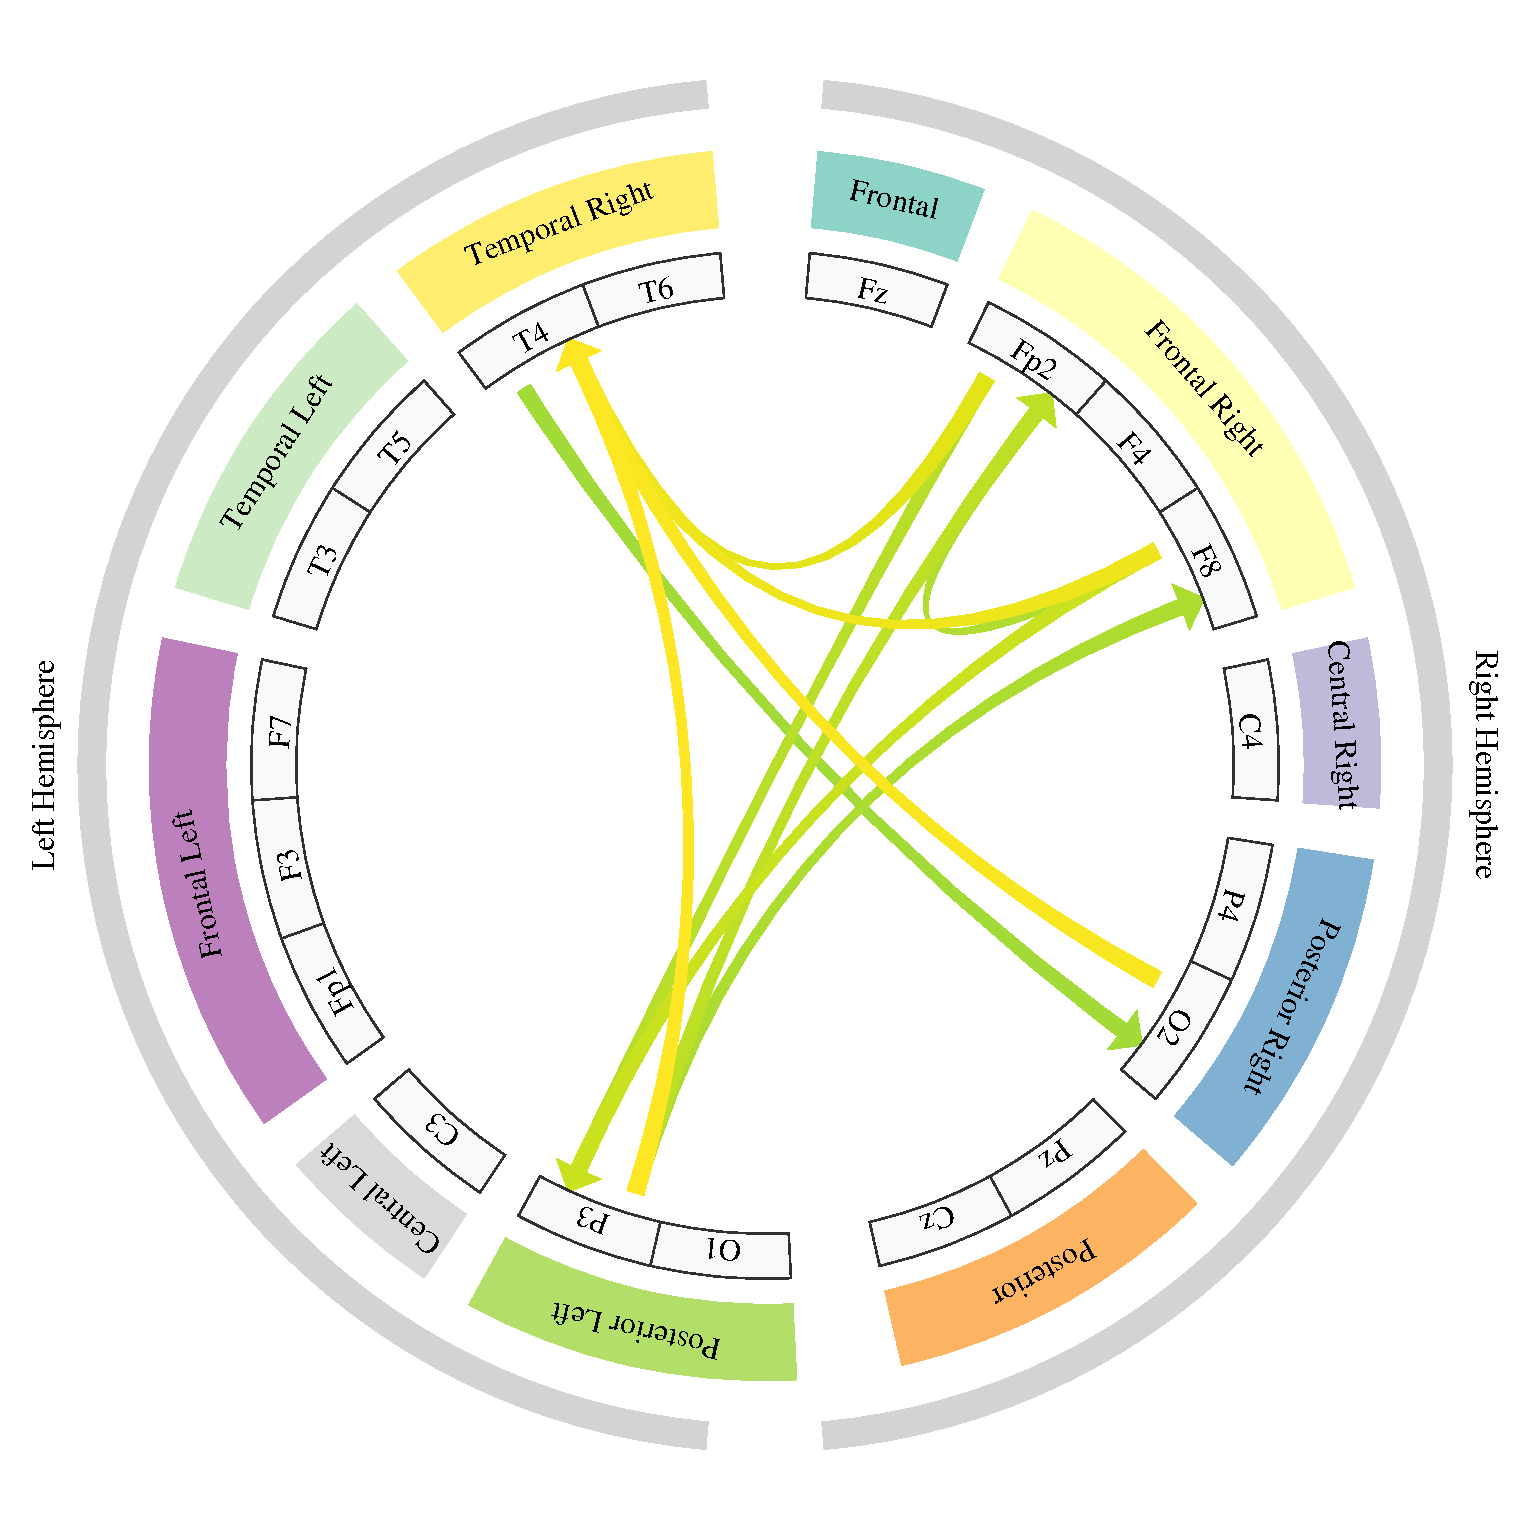
\includegraphics[
            width=\linewidth
        ]{Figures/misclassified_tdah_v27p_normalized.pdf}

        \vspace{1mm}

        {\small
        (b) Misclassified \gls{adhd} (\texttt{Sv27p}).}
    \end{minipage}
    \hfill
    \begin{minipage}[c]{0.045\textwidth}
        \centering

        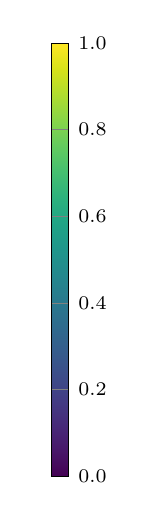
\begin{tikzpicture}
            \begin{axis}[
                hide axis,
                scale only axis,
                width=0pt,
                height=5.5cm,
                colormap/viridis,
                point meta min=0,
                point meta max=1,
                colorbar,
                colorbar style={
                    height=5.5cm,
                    width=0.22cm,
                    ytick={0,0.2,0.4,0.6,0.8,1},
                    yticklabels={0.0,0.2,0.4,0.6,0.8,1.0},
                    yticklabel style={
                        font=\scriptsize
                    }
                }
            ]

            \addplot[
                draw=none,
                point meta=explicit
            ]
            coordinates {
                (0,0) [0]
                (1,1) [1]
            };

            \end{axis}
        \end{tikzpicture}
    \end{minipage}

    \caption{
        Directed Transfer Entropy connectivity patterns for
        representative misclassified subjects.
        Only the top 5\% of the strongest directed connections are shown.
        Arrow direction indicates the estimated direction of information
        transfer, while color represents the normalized TE magnitude
        using a shared range.
    }

    \label{fig:misclassified_subjects_te}
\end{figure}
%----------------------------------------------------------
\subsection{Summary}
\label{sec:Conclu3}

In this chapter, we proposed \gls{ctenet}, an end-to-end architecture that extends the kernel-based Transfer Entropy (TE) framework through Transformer-based contextualization for pediatric attention-deficit/hyperactivity disorder (\gls{adhd}) classification. Building on the directed-dependency modeling developed with \gls{tektenet}, the proposed architecture integrates global contextualization, channel-wise nonlinear temporal filtering, Takens delay-coordinate reconstruction, and differentiable kernel TE estimation. This combination provides a supervised representation of nonlinear, time-delayed, and directed predictive dependencies while enabling the inspection of how \gls{eeg} Windows are organized within and across participants.

The experimental evaluation involved 120 children, five fixed subject-wise folds, and ten random training repetitions. \gls{ctenet} achieved a window-level accuracy of $80.9 \pm 1.7\%$ and a participant-level accuracy of $83.4\%$ (95\% CI: 78.2--88.2), with a participant-level ROC-AUC of $90.2\%$ (95\% CI: 85.1--94.6). These results support competitive classification performance under an evaluation in which test participants were absent from the corresponding training and validation subsets. Participant-level comparisons did not establish statistically significant differences from \gls{eeg}Net, ShallowConvNet, T-GARNet, or IMC-BGT after Holm correction, whereas the comparison with MultiStream favored \gls{ctenet}. Accordingly, the contribution is supported by the combination of predictive performance and an explicit directed-connectivity representation, without implying universal superiority over the evaluated classifiers.

The ablation analysis clarified the roles of the principal architectural components. Removing the Transformer produced the largest performance reductions, with a significant participant-level difference in favor of the complete model. Replacing the TE module with temporal mean pooling also reduced the point estimates, although the participant-level difference was not statistically significant. These findings support the predictive contribution of global contextualization and more moderate evidence for the incremental predictive benefit of TE. The TE module nevertheless supplies the nonlinear, delayed, and directed representation that enables the subsequent connectivity and feature-space analyses.

The representation analysis showed progressively more favorable class organization across the learned stages. The TE representation achieved the highest window- and centroid-level silhouette coefficients and the lowest normalized within-subject dispersion. Relative to raw \gls{eeg}, the median dispersion reduction was $38.35\%$, with lower dispersion in 76 of the 120 participants. The direction of this result persisted across the evaluated PCA dimensionalities and the cosine-distance analysis without PCA. These controls support consistency across the tested comparison spaces, although they do not establish independence from representation-specific standardization. Thus, the findings indicate that a discriminatively learned directed-connectivity space can reduce window-specific variability while retaining class-related structure.

Complementary connectivity analyses characterized both the interpretability and the stability of this representation. Across participants, the mean window-to-remaining-window Spearman correlation was $0.743$, whereas the mean Jaccard similarity for the strongest $10\%$ of connections was $0.492$. The overall ranking of connections was therefore more consistent across windows than the exact membership of the strongest subset. Selected individual maps illustrated different organizations in correctly and incorrectly classified cases, but did not establish population-level biomarkers. Because the Transformer contextualizes the channel representations before TE estimation, these coefficients describe directed predictive dependencies between learned channel-indexed coordinates, rather than direct interactions between anatomically localized cortical sources.

The sensitivity analyses also delineated the scope of the findings. Frequency filtering combined with quality screening reduced participant-level performance, while common average reference preserved classification performance but substantially changed the learned connections. Predictive robustness and connectivity stability must therefore be assessed separately. Together with the single-cohort design, unavailable participant-linked demographic and medication information, and the need for fully nested model selection, these findings limit clinical and physiological generalization. Overall, this chapter advances the thesis from directed-dependency estimation toward contextualized and inspectable \gls{eeg} representation learning, providing proof-of-concept evidence in a pediatric classification task that complements the preceding motor-imagery studies.